%% BioMed_Central_Tex_Template_v1.06
%%                                      %
%  bmc_article.tex            ver: 1.06 %
%                                       %

%%IMPORTANT: do not delete the first line of this template
%%It must be present to enable the BMC Submission system to
%%recognise this template!!

%%%%%%%%%%%%%%%%%%%%%%%%%%%%%%%%%%%%%%%%%
%%                                     %%
%%  LaTeX template for BioMed Central  %%
%%     journal article submissions     %%
%%                                     %%
%%          <8 June 2012>              %%
%%                                     %%
%%                                     %%
%%%%%%%%%%%%%%%%%%%%%%%%%%%%%%%%%%%%%%%%%


%%%%%%%%%%%%%%%%%%%%%%%%%%%%%%%%%%%%%%%%%%%%%%%%%%%%%%%%%%%%%%%%%%%%%
%%                                                                 %%
%% For instructions on how to fill out this Tex template           %%
%% document please refer to Readme.html and the instructions for   %%
%% authors page on the biomed central website                      %%
%% http://www.biomedcentral.com/info/authors/                      %%
%%                                                                 %%
%% Please do not use \input{...} to include other tex files.       %%
%% Submit your LaTeX manuscript as one .tex document.              %%
%%                                                                 %%
%% All additional figures and files should be attached             %%
%% separately and not embedded in the \TeX\ document itself.       %%
%%                                                                 %%
%% BioMed Central currently use the MikTex distribution of         %%
%% TeX for Windows) of TeX and LaTeX.  This is available from      %%
%% http://www.miktex.org                                           %%
%%                                                                 %%
%%%%%%%%%%%%%%%%%%%%%%%%%%%%%%%%%%%%%%%%%%%%%%%%%%%%%%%%%%%%%%%%%%%%%

%%% additional documentclass options:
%  [doublespacing]
%  [linenumbers]   - put the line numbers on margins

%%% loading packages, author definitions

%\documentclass[twocolumn]{bmcart}% uncomment this for twocolumn layout and comment line below
\documentclass{bmcart}

%%% Load packages
%\usepackage{amsthm,amsmath}
%\RequirePackage{natbib}
%\RequirePackage{hyperref}
\usepackage[utf8]{inputenc} %unicode support
\usepackage{url}
\usepackage{graphics}
\usepackage{graphicx}
\usepackage{multirow}
%\usepackage[applemac]{inputenc} %applemac support if unicode package fails
%\usepackage[latin1]{inputenc} %UNIX support if unicode package fails


%%%%%%%%%%%%%%%%%%%%%%%%%%%%%%%%%%%%%%%%%%%%%%%%%
%%                                             %%
%%  If you wish to display your graphics for   %%
%%  your own use using includegraphic or       %%
%%  includegraphics, then comment out the      %%
%%  following two lines of code.               %%
%%  NB: These line *must* be included when     %%
%%  submitting to BMC.                         %%
%%  All figure files must be submitted as      %%
%%  separate graphics through the BMC          %%
%%  submission process, not included in the    %%
%%  submitted article.                         %%
%%                                             %%
%%%%%%%%%%%%%%%%%%%%%%%%%%%%%%%%%%%%%%%%%%%%%%%%%


%\def\includegraphic{}
%\def\includegraphics{}



%%% Put your definitions there:
%\startlocaldefs
%\endlocaldefs


%%% Begin ...
\begin{document}

\begin{frontmatter}

\begin{fmbox}
\dochead{Research}

\title{An Investigation of the Performance of UK ISP Web Filters}

\author[
   addressref={lancs},                   % id's of addresses, e.g. {aff1,aff2}
   corref={lancs},                       % id of corresponding address, if any
   %noteref={n1},                        % id's of article notes, if any
   email={m.rowe@lancaster.ac.uk}   % email address
]{\inits{MR}\fnm{Matthew} \snm{Rowe}}
\author[
   addressref={org},                   % id's of addresses, e.g. {aff1,aff2}
   corref={org},                       % id of corresponding address, if any
   %noteref={n1},                        % id's of article notes, if any
   email={richard@openrightsgroup.org}   % email address
]{\inits{RK}\fnm{Richard} \snm{King}}

\address[id=lancs]{%                           % unique id
  \orgname{Data Science Group, School of Computing and Communications}, % university, etc
  \street{Lancaster University},                     %
  \postcode{LA1 4WA}                                % post or zip code
  \city{Lancaster},                              % city
  \cny{UK}                                    % country
}
\address[id=org]{%                           % unique id
  \orgname{Open Rights Group}, % university, etc
  \street{Free Word Centre, 60 Farringdon Road},                     %
  \postcode{EC1R 3GA}                                % post or zip code
  \city{London},                              % city
  \cny{UK}                                    % country
}

\end{fmbox}% comment this for two column layout

\begin{abstractbox}

\begin{abstract} % abstract
To do
\end{abstract}


\begin{keyword}
\kwd{sample}
\kwd{article}
\kwd{author}
\end{keyword}

% MSC classifications codes, if any
%\begin{keyword}[class=AMS]
%\kwd[Primary ]{}
%\kwd{}
%\kwd[; secondary ]{}
%\end{keyword}

\end{abstractbox}
%
%\end{fmbox}% uncomment this for twcolumn layout

\end{frontmatter}

%%%%%%%%%%%%%%%%%%%%%%%%%%%%%%%%%%%%%%%%%%%%%%
%%                                          %%
%% The Main Body begins here                %%
%%                                          %%
%% Please refer to the instructions for     %%
%% authors on:                              %%
%% http://www.biomedcentral.com/info/authors%%
%% and include the section headings         %%
%% accordingly for your article type.       %%
%%                                          %%
%% See the Results and Discussion section   %%
%% for details on how to create sub-sections%%
%%                                          %%
%% use \cite{...} to cite references        %%
%%  \cite{koon} and                         %%
%%  \cite{oreg,khar,zvai,xjon,schn,pond}    %%
%%  \nocite{smith,marg,hunn,advi,koha,mouse}%%
%%                                          %%
%%%%%%%%%%%%%%%%%%%%%%%%%%%%%%%%%%%%%%%%%%%%%%

%%%%%%%%%%%%%%%%%%%%%%%%% start of article main body
% <put your article body there>

%%%%%%%%%%%%%%%%
%% Background %%
%%
\section*{Introduction}

%Context/Problem
%-Introduction of UK ISP Web Filters
%-Questions over:
%--the need for this (cite ofcom survey states)
%--their accuracy, given that the ISPs use third-party systems or categorisations
%--how they can be held to account
%--who is responsible for their oversight (this is left vague)

In 2013, the United Kingdom government instructed all UK-based Internet Service Providers (ISPs) to provide new customers with an `\textit{unavoidable}' choice: \textit{to turn on web filtering, or not}. 
This was presented to such customers as a web-based form to which the customers provided their answer; and should the customer select \textit{yes} then for certain ISPs additional questions would be asked about the level of filtering required.
Such web filtering was mandated in order to protect children from adult content (e.g. pornography, alcohol, and drugs), and to ensure that they can browse and use the Web in a safe manner.
However after one year of the provision of such filters, an Ofcom report\footnote{\url{http://stakeholders.ofcom.org.uk/internet/internet-safety-2}} found that for new ISP customers, who were offered the choice of filtering uptake ranged across ISPs from only 5\% to 36\%.

During the period since the filters' inception, various news outlets have reported on examples of `\textit{overblocking}' by ISPs - where sites are blocked that should not have been - such as sexual health advice blogs, charity web sites, addiction-support sites, and politics-related web sites and opinion blogs.
This has led to questions being raised as to the accuracy of the filters, what they are blocking that they should not be (\textit{overblocking}), and what sites they are not filtering out that they should be (\textit{underblocking}).
As such, this growing discourse is  calling into question the \textit{efficacy} of the filters and the degree of censorship that they are enabling.
Despite such questions being raised, at present little is known of how effective the filters are, as the ISPs do not report on their accuracy.
Motivated by this current lack of understanding, in this paper we investigate the following three research questions:

\begin{enumerate}
	\item \textbf{RQ1}: How can we understand how UK ISP Web Filters function, and how accurate they are?
	\item \textbf{RQ2}: How reliable are the filters at blocking content, in terms of both overblocking and underblocking across different categories of sites? And are there certain categories of web sites that are error prone?
	\item \textbf{RQ3}: How long does it take an ISP to fix an error?
\end{enumerate}

In order to investigate the above questions, we present a study of both UK ISPs and Mobile Service Providers' (MSPs) filters using data collected by the Open Rights Group\footnote{A non-profit UK-based organisation who campaign for and work to promote digital rights} as part of their Blocked.org.uk\footnote{\url{https://www.blocked.org.uk/}} project.
The aim of the project was to \textit{probe} a range of Internet (ISPs) and Mobile Service Providers (MSPs) with a collection of URLs and collect examples of blocked and unblocked web sites.
In performing this study, we follow a \textit{data science} approach by first performing exploratory analysis at the \textit{macro} level of what domains are commonly blocked and what categories of sites are blocked by the filters, before then investigating the accuracy of the filters and to identify any categories of sites that are routinely \textit{overblocked} and \textit{underblocked}, thus performing a relational study between filters and their accuracy, and site categories.

This paper makes the following contributions:
\begin{enumerate}
	\item An empirical characterisation of UK ISPs' and MSPs' filtering accuracy over time.
	\item Evidence of overblocked and underblocked sites by UK ISPs and MSPs.
	\item A computational framework harnessing Apache Spark for parallelised processing of probe data.
\end{enumerate}

This work is the first to investigate the performance of UK ISP web filters and to provide evidence of both overblocking and underblocking.
For that reason, the work has huge potential for implications on the domains of digital rights and censorship, and also data science in the methodology that we follow in investigating web filters' performance through data - so-called `\textit{data-driven digital accountability}'. 
We begin this paper by first explaining related works study web filtering technology and web censorship, and the inherent impact of both; before then moving on to outlining which Internet and Mobile Service Providers.
We follow this up by describing how the \textit{probe} system works for monitoring web filters, before then presenting evidence of what domains and categories of sites are being blocked and by whom.
In the proceeding sections we then explain how we gauge filter accuracy, present qualitative examples of incorrectly blocked sites, and investigate how quickly an ISP responds to fix an incorrect block.
In order to provide full transparency of how this paper's results and findings were derived, both the software used to analyse the web filters and the results from our analyses are available on the Open Rights Group's Github repository.\footnote{\url{https://github.com/openrightsgroup/cmp-analysis}}





\section*{Related Work}
To date, the investigation and exploration of web filtering has been largely concentrated in the literature around \textit{censorship}, despite the evocative-nature of the term.
For instance, early work by Adkeniz \cite{akdeniz2001internet} argued against censorship as rhetoric was emerging around the need to censor the Internet - largely in order to protect under-18s from being exposed to potentially harmful content.
Adkeniz's view was that free speech must be maintained here, and that filtering must only be performed with the correct safeguards in place - to ensure correct application.
McIntyre and Scott \cite{mcintyre2008internet} expanded over this line of work by examining the role of web filtering and governance.
The authors argued that while existing forms of censorship are mandated by politicians, web filtering follows a different route and involves different actors (e.g. third-party companies), thereby reducing the transparency surrounding the process and the accountability that accompanies this.

The rise in state censorship of the Internet in countries such as China, Syria, Saudia Arabia, and Turkey, has led to a body of work attempting to understand what filtering mechanisms are at play, and whether and how such mechanisms are being circumvented.
For instance, Verkamp \& Gupta \cite{verkamp2012inferring} looked at different mechanisms by which web censorship takes place throughout different countries (e.g. Turkey, Saudi Arabia).
The authors mapped out the landscape of filtering mechanisms, finding: different triggers (e.g. hostname, IP address), and modes of censorship application (e.g. filtering requests, modifying responses); in doing so, the authors were able to devise a system to probe which URLs were blocked and by whom.
Similar work by Dalek et al. \cite{dalek2013method} presented a method to detect which filtering technology is being used for censorship, again focussing on state-level censorship.
Their approach demonstrated that a combination of HTTP headers' keywords and path information can be used to identify known filtering technologies being used (e.g. Netsweeper).

The expanse of web filtering across states has seen the creation of community-led internet-wide initiatives to monitor censorship.
One such initiative is the OpenNet Initiative (ONI)\footnote{\url{https://opennet.net/}} run with the intention of gathering evidence of censorship and providing the technical infrastructure to monitor the use of Internet filtering.
Work by Crete et al. \cite{crete2013not} used data provided by ONI to understand how censorship is performed and why this takes place.
The authors described a by-product of censorship known as `\textit{collateral filtering}' where filtering leads to other content being blocked inadvertently - i.e. so-called overblocking.
This notion of \textit{collateral filtering} is reinforced by Murdoch \& Roberts \cite{murdoch2013internet} when examining the role of censorship and its perceptions, as they state that: ``\textit{... over-blocking is an underhanded attempt to avoid criticism, but other times it proves to be a mistake resulting from overzealous interpretations of rules or collateral damage due to technical limitations in censorship techniques.}''
Similar to ONI, the Tor project's Open Observatory of Network Interference (OONI) software \cite{ooni2015} has been used throughout community-led initiatives to monitor which URLs are blocked, where and when.
While Aceto et al. \cite{aceto2015monitoring} provided a platform known as the User-based Internet Censorship Analysis (UBICA) platform to allow users to run tests over their ISP connection to ascertain what is being blocked.
Given the myriad ways in which web filtering can function (DNS-tampering, keyword blocking), we refer the reader to the detailed and comprehensive review of approaches for detecting web filtering by Aceto and Pescape \cite{aceto2015internet} for further information.

The study of web filtering and its mechanisms transcends various layers including the state, as in \cite{verkamp2012inferring, dalek2013method, crete2013not, aceto2015monitoring}, and organisations.
For the latter, Esnaashari et al. \cite{esnaashari2014restrictions} focussed on web filtering in New Zealand throughout organisations that provide web access- e.g. in libraries, cafes, etc..
Unsurprisingly, the authors found that different organisations blocked different types of content and applied different levels of filtering.

\subsection*{Computing filter accuracy}
One of the core aims of our work is to understand how well UK ISPs and MSPs perform web filtering, thereby allowing the public to understand how reliable web filtering is.
Prior work has sought to gauge the degree of filtering, however the limitation to state censorship restricts researchers from knowing what \textit{should} be blocked - and thus allowing the accuracy of filters to be gauged.
One of the first works in this direction was produced by researchers from Google's Zion VLab \cite{Anonymous:2012:CDI:2317307.2317311} who examined the extent to which collateral damage occurs through state-level censorship programmes.
The authors found evidence of DNS injectors along query transit paths, meaning that routing of hostname responses is injected as a form of filtering - happening within the transit-phase of a hostname being queried and then resolved.
More recent work by Nabi \cite{nabi2014censorship} investigated the uptake of certain web sites in countries where they have been blocked.
The author demonstrated that sites that had been publicly declared as blocked actually increased in their visits post-blocking, thereby suggesting evidence of a `\textit{Streisand effect}'.\footnote{The \textit{Streisand Effect} occurs when a given party attempts to block, or censor, information being published, and in doing so raises awareness of said information - thereby having the opposite effect of that intended.}

Despite the wide body of work covering the detection of filtering approaches and their usage across various countries, we could only find one piece of work that empirically characterised web filters' accuracy.
The work in question, by Stark \cite{stark2007effectiveness}, used a sample of URLs categorised as either adult or clean, passed these URLs through various home PC web filters (e.g. McAfee, CyberPatrol) and then computed: (i) the underblocking percentage (i.e. the percentage of URLs that should have been blocked that weren't), and; (ii) the overblocking percentage (i.e. the percentage of URLs that were blocked that should not have been).
Stark's results derived underblocking percentages ranging from 6.2\% to 43.4\%  for various filters, and from 0.4\% to 20.7\% for overblocking; thereby indicating that filters perform better at minimising incorrect blocks than detecting what it should be blocked.
As of writing this paper, we were unable to find any literature that examined the performance of UK ISP and MSP web filters, nor their uptake - aside from the Ofcom Internet Safety report in 2014.\footnote{\url{http://stakeholders.ofcom.org.uk/internet/internet-safety-2}}

The above works demonstrate that researchers have largely concentrated on understanding how state and organisation-level censorship takes place, and the myriad ways in which filtering operates at a technical level.
As such, existing work has yet to quantify web filters' accuracy and the degree to which `\textit{collateral filtering}' is evident (i.e. overblocking and underblocking); we believe that this is largely due to the lack of prescribed lists of gold standard blocks.
In this paper we present for the first time evidence of such collateral filtering and provide empirical evidence of how accurate ISP and MSP web filters are.
This is enabled, as we will detail below, by examining ISPs' and MSPs' descriptions of their filters and their intended categories of blocked sites, which we operationalise through modelling filters as \textit{pseudo-classifiers} and computing their accuracy against a gold-standard.


\section*{Studied Internet and Mobile Service Providers}
The United Kingdom's telecommunications market is one of the biggest in the world, and consumers are provided with a range of Internet Service Providers and Mobile Service Providers to choose from.
In order to provide data for our analysis, we used both ISPs and MSPs that had the largest consumer bases in the country.
For the ISPs we examined the web filtering of: BT, PlusNet, Sky, TalkTalk, and VirginMedia; while for the MSPs we examined the web filtering of: EE, O2, T-Mobile, VirginMobile, and Vodafone.
We now describe the filtering technologies and available filter settings of each.

\subsubsection*{Internet Service Providers' Filters}
\paragraph{BT.}
BT provide a system known as `\textit{BT parental controls}'\footnote{\url{http://www.productsandservices.bt.com/products/manage-broadband-extras/}} which uses DNS-based blocking of URLs.
The system utilises site categorisation information from Nominum\footnote{\url{http://nominum.com/}} by looking up requested hostnames and blocking any requests for URLs from banned lists.
BT provide three levels of filtering once turned on: (i) \textit{light}, which blocks pornography, obscene and tasteless, hate and self-harm, drugs, alcohol and tobacco, and dating; (ii) \textit{moderate}, which blocks all of the light filter settings plus nudity, weapons and violence, gambling, and social networking, and finally; (iii) \textit{strict}, which blocks all of the above plus fashion and beauty, file-sharing, games, and media streaming.

\paragraph{PlusNet.}
Use network-level filtering of piracy sites, and at present do not filter any adult web content.

\paragraph{Sky.}
Sky provide a filtering system known as `\textit{Sky Broadband Shield}' that also uses DNS-based blocking of URLs, however unlike BT, Sky's system uses site categorisation information provided Symantec and their Rulespace Web Content categorisation system.\footnote{\url{http://www.symantec.com/page.jsp?id=rulespace}} 
Similar to BT, Sky offer three levels of categorisation: (i) \textit{18} which blocks malware sites; (ii) \textit{13} which blocks cyber-bullying, pornography, suicide and self-harm, drugs, dating, and malware sites, and; (iii) \textit{PG} which blocks all of the above plus social networking and online gaming.

\paragraph{Talk Talk.}
Talk Talk provide a filtering system known as HomeSafe\footnote{\url{http://www.talktalk.co.uk/security/homesafe-demo.html}}, however unlike BT and Sky, this system using Deep-Packet Inspection to examine URLs being visited by users.
The filter includes the setting of a \textit{Kids Safe} filter that allows certain categories of sites to be blocked: Dating, Drugs, Alcohol and Tobacco, File Sharing Sites, Gambling, Games, Pornography, Social Networking, Suicide and Self-Harm, and Weapons and Violence.

\paragraph{VirginMedia.} 
This ISP provides a a system known as `\textit{Web Safe}'\footnote{\url{http://my.virginmedia.com/my-apps/websafe.html}} that is a DNS-based system which matches requested URLs with known blocked URLs in a DNS-lookup table.
As with BT, VirginMedia also use site categorisation information from Nominum.
From VirginMedia's web site, it is not clear what \textit{Web Safe} blocks, therefore such categories of sites were obtainted from the OFCOM Internet Safety Measures report from 2014.\footnote{\url{http://stakeholders.ofcom.org.uk/binaries/internet/internet_safety_measures_2.pdf}}


\subsubsection*{Mobile Service Providers' Filters}
Unlike Internet Service Providers, Mobile Service Providers can sell their products (e.g. pay as you go phones) to people under the age of 18.
As a result, customers are able to access content that may not be deemed suitable for their age group.
Below we describe the filtering approaches taken by the MSPs and what they block.
In general, MSPs have filtering turned on by \textit{default} and require customers to turn off the filters by verifying their age.

\paragraph{EE and T-Mobile.}
Both EE and T-Mobile use a system known as `\textit{Content Lock}'\footnote{\url{http://ee.co.uk/help/safety-and-security/my-digital-life/content-lock-and-orange-safeguard}}.
This system has one filter setting that blocks categories of sites including: alcohol, anonymisers, criminal skills, drugs, gore, hacking, hate, pornography, self harm, sex advice, suicide, tobacco, and violence.

\paragraph{O2.}
Use a filtering system known as `\textit{O2 18+}' with default-on setting, so filtering is always applied.
Symantec RuleSpace\footnote{\url{http://www.symantec.com/page.jsp?id=rulespace}} is used for site categorisation, and anything that is classed as `\textit{Adult}' by the BBFC (British Board of Film Classification)\footnote{\url{http://www.bbfc.co.uk/}} is blocked.

\paragraph{Three.}
As with O2, blocks any sites categorised as Adult, and therefore suitable for those over the age of 18, by the BBFC.

\paragraph{Vodafone.}
Vodafone provider filtering through their `\textit{Content Control}'\footnote{\url{http://support.vodafone.co.uk/Internet/Content-control-and-Vodafone-Guardian/38914008/How-can-I-switch-off-content-control-so-I-can-access-age-restricted-content-on-the-internet.htm}} system, with categorisation of web sites provided by Symantec.
Filtering is default-on, meaning that customers must remove filtering manually by proving that they are over 18.
There is only one level of filtering used here and this blocks: chat and dating services, erotica, gambling, and violent games.


\section*{Monitoring Web Filters}
We now move onto the crux of our work.
In order to understand how \textit{well} ISPs' and MSPs' web filters perform we first need to gather information about which URLs each filter has blocked and when this took place.
For this we used data provided by the Open Rights Group as part of their Blocked.org.uk project: below, we describe hos the project's probe system functions before then moving on to describing the data that we collected.

% Richard - need your input in to this section
\subsection*{Blocked.org.uk Probe System}
-Explain the framework that was used for this
-Explain the submission interface and the use of the blocked portal to check what has been blocked and unblocked
-Gathering evidence of overblocking and underblocking
-Explain the settings of each filter - i.e. default settings for each

\subsection*{Data Captured}
For this paper we used data collected from the probe system up to the end of March 2015, thereby providing around 9 months' worth of data for analysis.
Figure \ref{fig:total-requests} shows the distribution of requests per day that were collected in our dataset - a single request consists of a URL being tested by a given filter at a given time, hence representing a unique record.
In total we collected 6,289,550 requests for URLs across the studied ISPs and MSPs; Table \ref{tab:dataset_summary} shows the requests per-ISP and per-MSP that were collected.


\begin{table}[h!]
\caption{Dataset of requests from Blocked.org.uk}
  \begin{tabular}{ l l c}
    \hline
     & Time Interval & Requests \\
    \hline
	BT & [July 2014, April 2015] & 877,768 \\
	PlusNet & [June 2014, April 2015]  & 876,218 \\
    Sky & [June 2014, April 2015] & 883,571 \\
    TalkTalk & [July 2014, April 2015] & 883,787 \\
	VirginMedia & [June 2014, April 2015] & 883,743 \\
	\hline    
	EE & [May 2014, March 2015] & 270,471 \\
	O2 & [May 2014, March 2015] & 495,429 \\
	Three & [May 2014, March 2015] & 282,017 \\
	T-Mobile & [April 2014, September 2014] & 483 \\
	Vodafone & [March 2014, March 2015] & 836,063 \\
    \hline
  \end{tabular}
  \label{tab:dataset_summary}
\end{table}

\begin{figure}[t]
\caption{\csentence{Number of URL requests made over time since the beginning of the project.}}
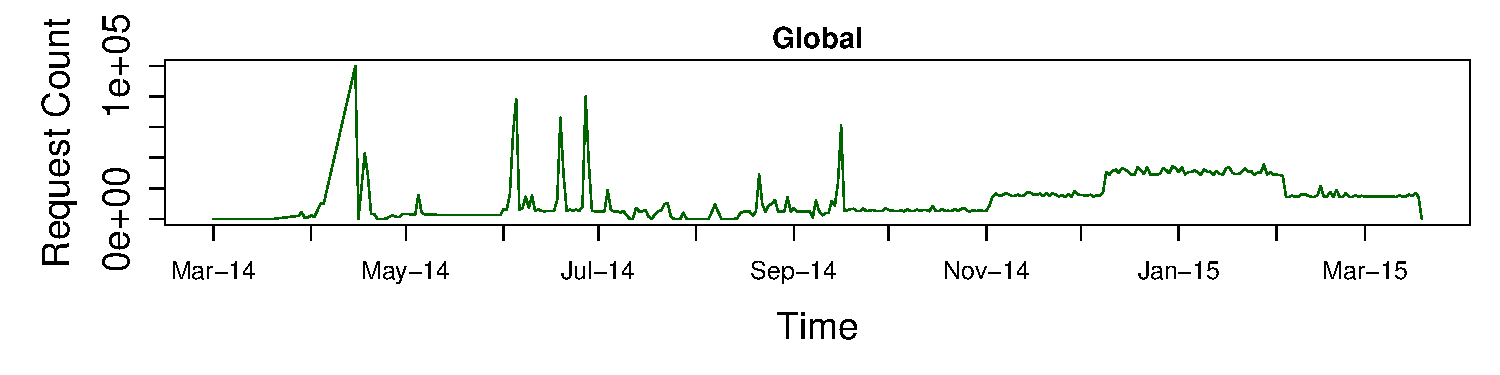
\includegraphics[width=0.9\textwidth]{imgs/ts-global-requests.pdf}
\label{fig:total-requests}
\end{figure}

Inspecting the per-ISP distributions of requests per day, as shown in Figure \ref{fig:broadband-requests}, we can see that we cover different time intervals for different ISPs with BT's and TalkTalk's collection starting later than PlusNet, Sky and VirginMedia.
Such differences in intervals were due to the slight delay in configuring the probe system for these connections. 

\begin{figure}[h!]
\caption{\csentence{Number of URL requests made per broadband ISP filter}}
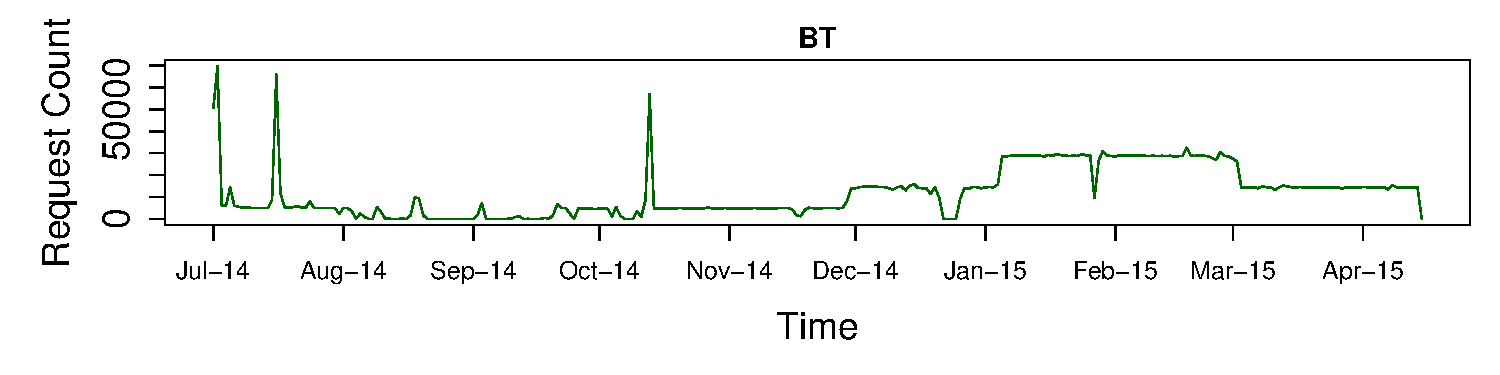
\includegraphics[width=0.49\textwidth]{imgs/BT-ts-requests.pdf}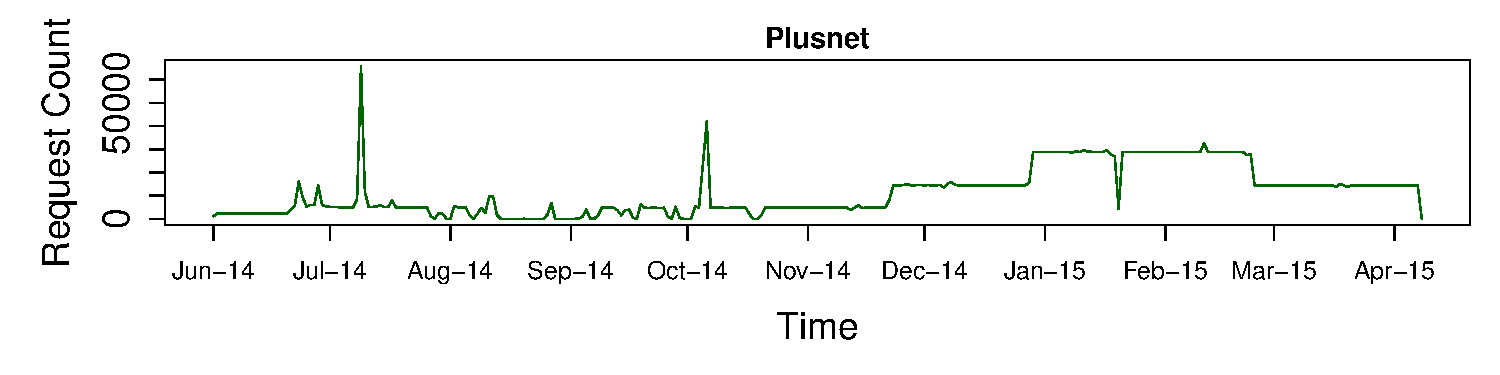
\includegraphics[width=0.49\textwidth]{imgs/Plusnet-ts-requests.pdf}
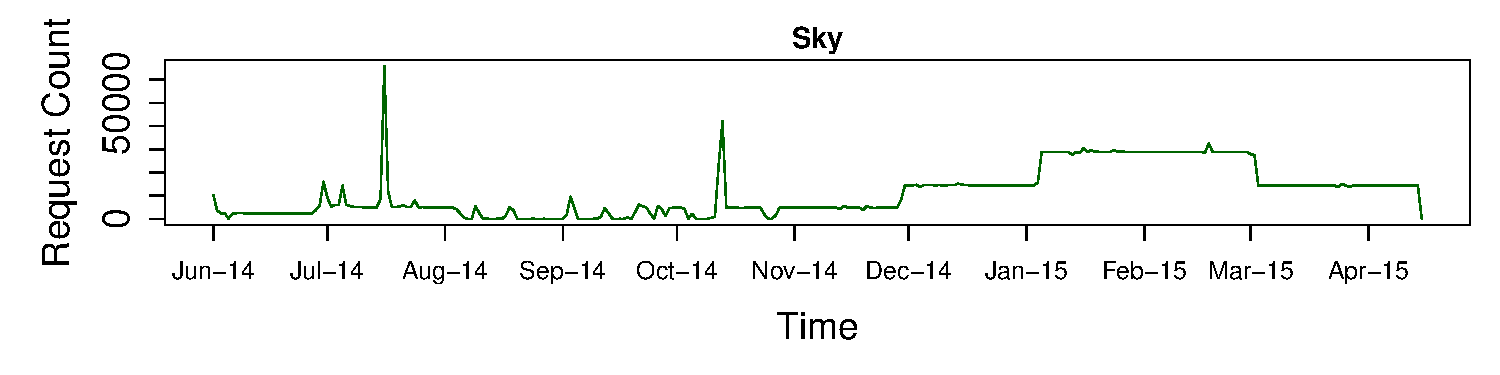
\includegraphics[width=0.49\textwidth]{imgs/Sky-ts-requests.pdf}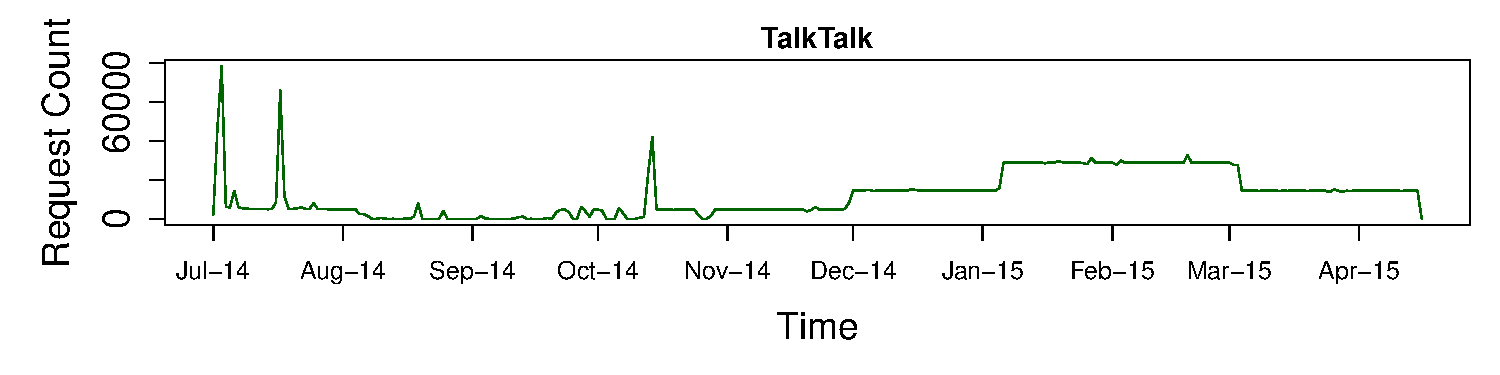
\includegraphics[width=0.49\textwidth]{imgs/TalkTalk-ts-requests.pdf}
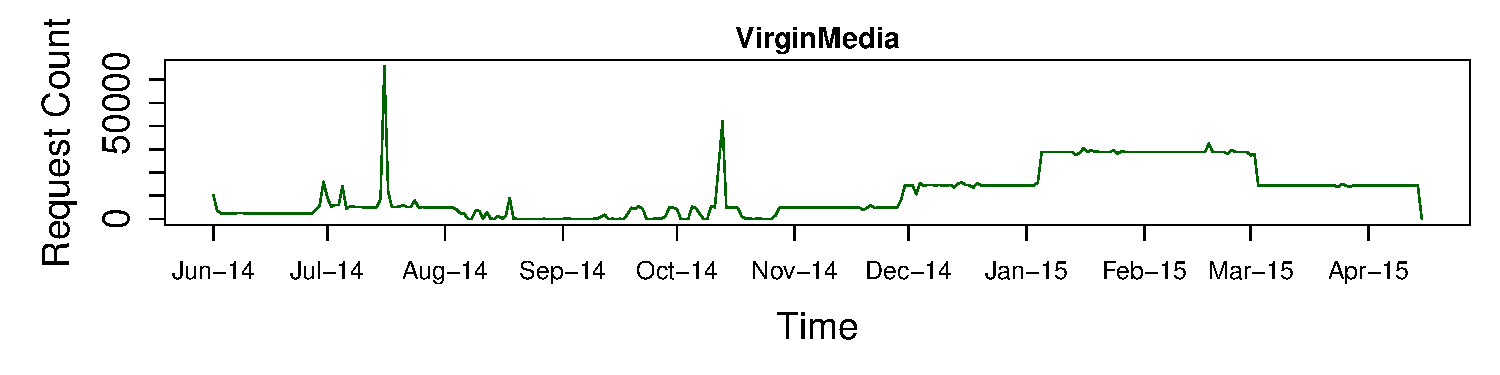
\includegraphics[width=0.49\textwidth]{imgs/VirginMedia-ts-requests.pdf}
\label{fig:broadband-requests}
\end{figure}

In a similar vein to the ISPs' plots, we can also inspect the distribution of requests per day for the MSPs - shown in Figure \ref{fig:mobile-requests}.
As with the ISPs, we observe that collections cover different time intervals: Vodafone collection spanning March 2014 to March 2015, EE, O2 and Three spanning May 2014 to March 2015, and T-Mobile spanning April 2014 to October 2014.
This latter MSP's probe had issues collecting requests and testing for blocks, therefore we do not use T-Mobile in our analysis - despite this we are able to analyse EE which uses the same underlying filtering technology.

\begin{figure}[h!]
\caption{\csentence{Number of URL requests made per mobile ISP filter}}
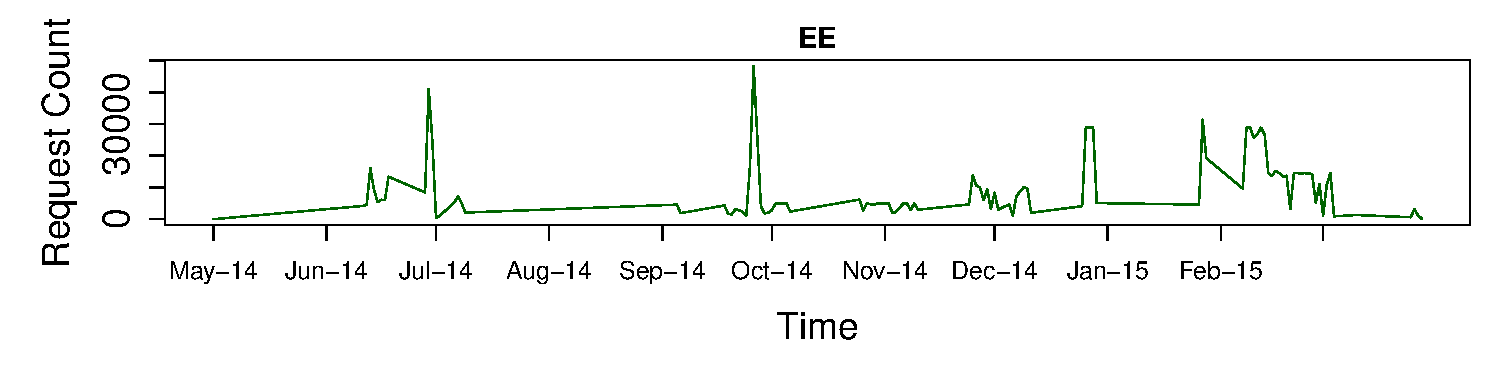
\includegraphics[width=0.49\textwidth]{imgs/EE-ts-requests.pdf}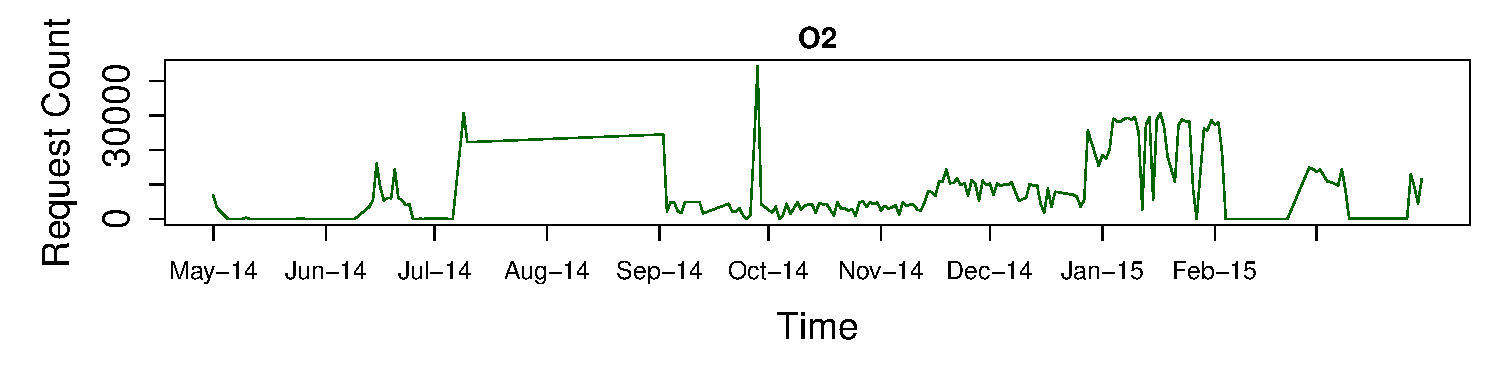
\includegraphics[width=0.49\textwidth]{imgs/O2-ts-requests.pdf}
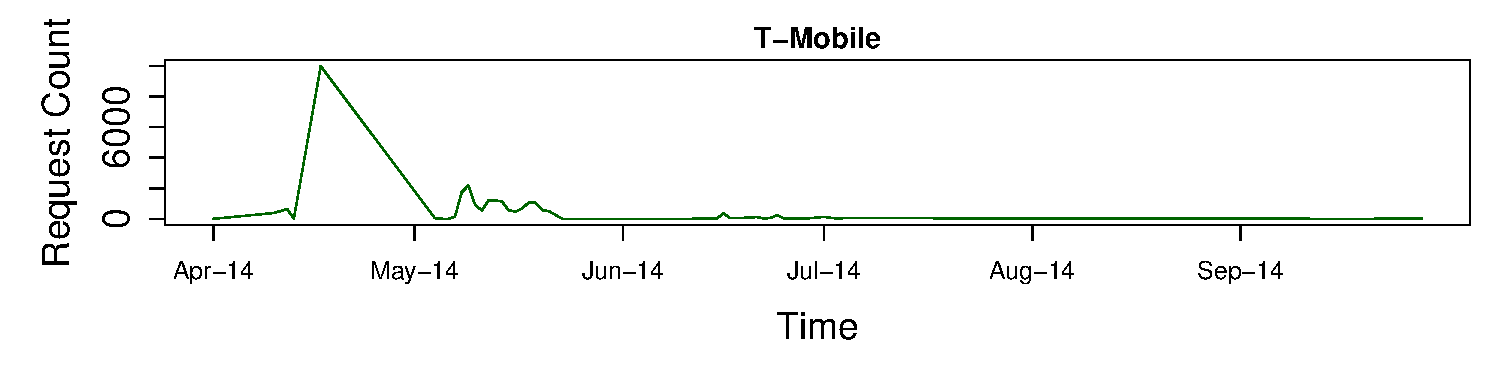
\includegraphics[width=0.49\textwidth]{imgs/T-Mobile-ts-requests.pdf}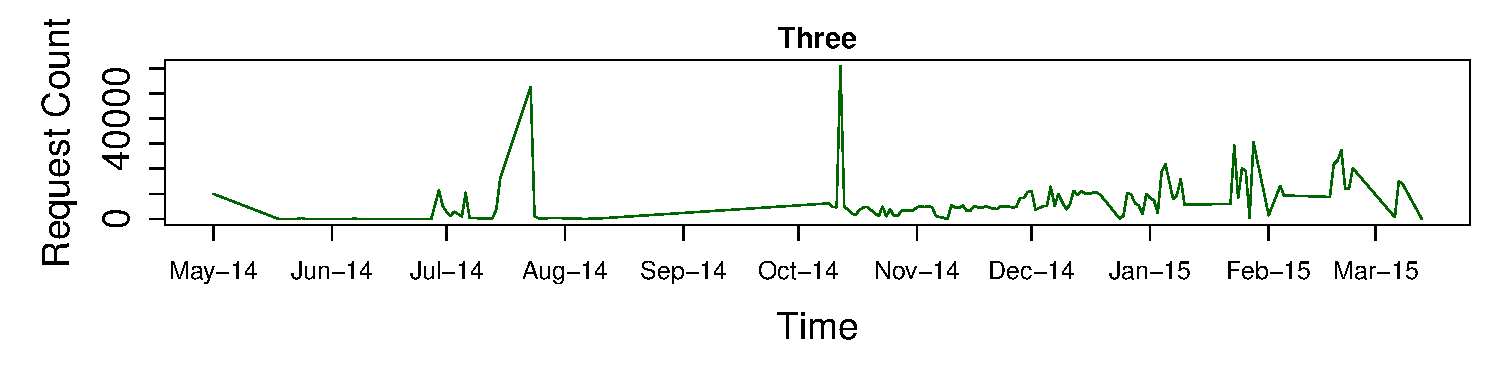
\includegraphics[width=0.49\textwidth]{imgs/Three-ts-requests.pdf}
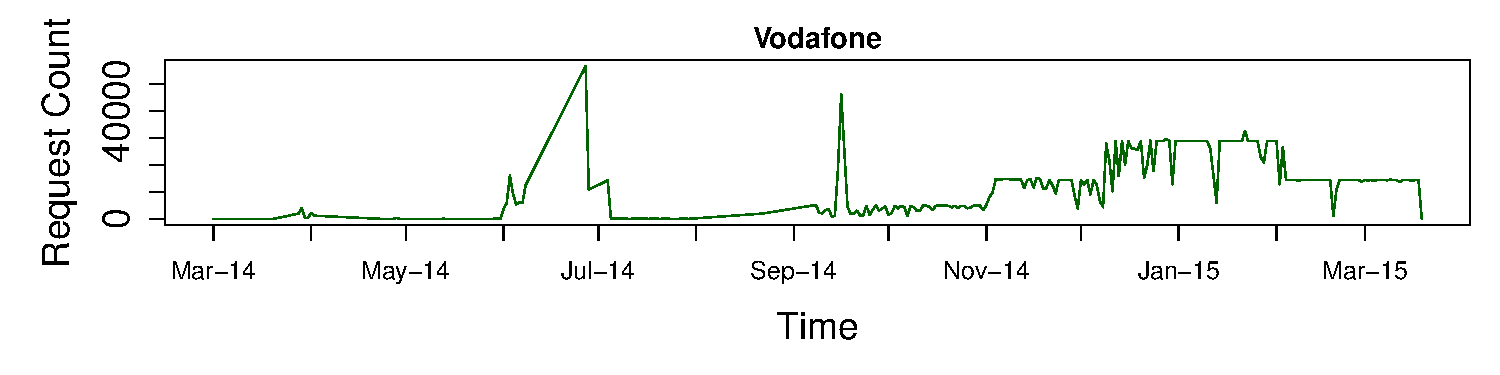
\includegraphics[width=0.49\textwidth]{imgs/Vodafone-ts-requests.pdf}
\label{fig:mobile-requests}
\end{figure}



\section*{Blocked Content}
This section begins our exploratory analysis of what has been blocked by the UK ISPs and MSPs.
We start by assessing the top-level URLs domains of blocked requests, before then moving on to examine the categories of blocked URLs.

\subsection*{Blocked Domains}
We began by investigating which domains had been blocked by Internet Service Providers.
To do this, we extracted the blocked requests for each ISP and then recorded the frequency distributions of the blocked URLs domains (e.g. \url{www.lancs.ac.uk/staff/rowem} would have domain \url{lancs.ac.uk}).

Figure \ref{fig:broadband-blocked-domains} shows the top-40 domains that are blocked by ISPs' filters. 
As PlusNet does not use filtering, we can see that the only URLs that are blocked are those related to file-sharing sites such as The Pirate Bay and similar platforms - these were served with a UK court order to be blocked in 2013.
For the remaining ISPs, the top-most domains that are blocked are pornography (e.g. \url{pornhub}, \url{xhamster}, etc.), and other adult-content sites (e.g. \url{4chan}).
Interestingly, we found that certain domains are picked up that we would not associate with adult content, such as \url{reddit}, \url{tumblr}, and (worryingly) \url{torproject}.

\begin{figure}[h!]
\caption{\csentence{Distributions of blocked domains for broadband ISPs} This presents which domains each ISP has blocked and the frequency distribution of those domains.}
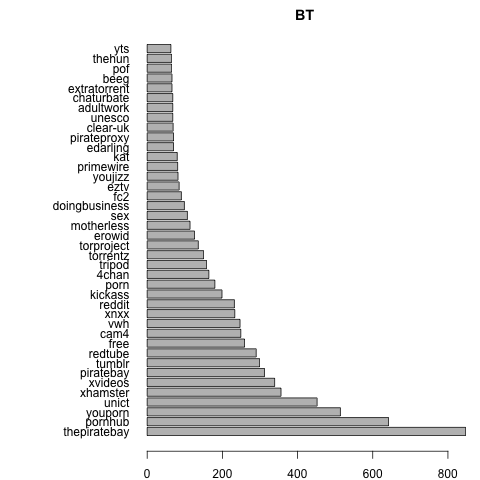
\includegraphics[width=0.49\textwidth]{imgs/BT-blocked-pages-to-date}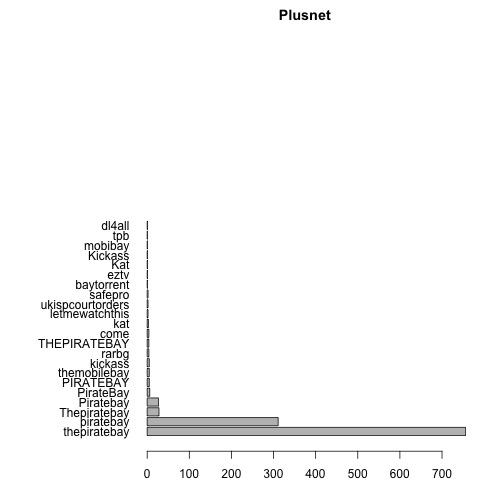
\includegraphics[width=0.49\textwidth]{imgs/Plusnet-blocked-pages-to-date}
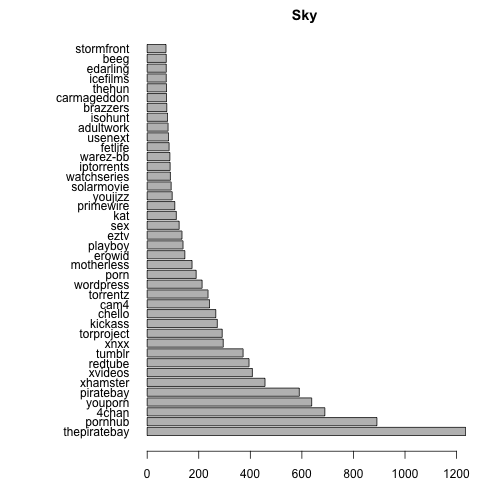
\includegraphics[width=0.49\textwidth]{imgs/Sky-blocked-pages-to-date.png}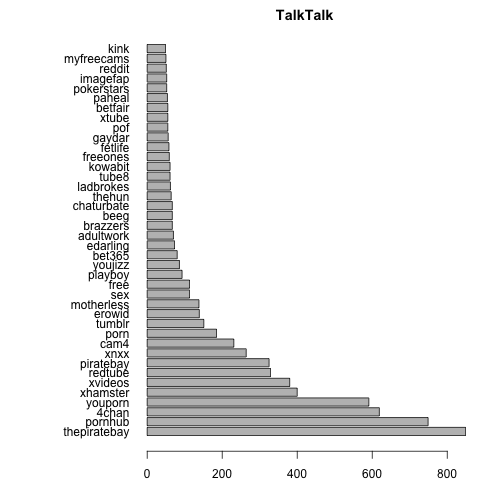
\includegraphics[width=0.49\textwidth]{imgs/TalkTalk-blocked-pages-to-date}
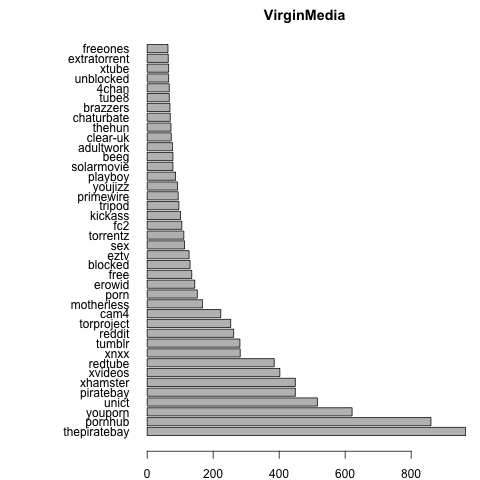
\includegraphics[width=0.49\textwidth]{imgs/VirginMedia-blocked-pages-to-date}
\label{fig:broadband-blocked-domains}
\end{figure}

Inspection of the top-40 blocked domains of blocked sites by MSPs (in Figure \ref{fig:mobile-blocked-domains}) reveals similar findings to that of the ISPs: with pornography and adult-content sites being blocked, yet with other domains of sites that are not normally associated with adult-content also being blocked (e.g. \url{torproject}, \url{tripod}, \url{wordpress}).

\begin{figure}[h!]
\caption{\csentence{Distributions of blocked domains for mobile ISPs} This presents which domains each ISP has blocked and the frequency distribution of those domains.}
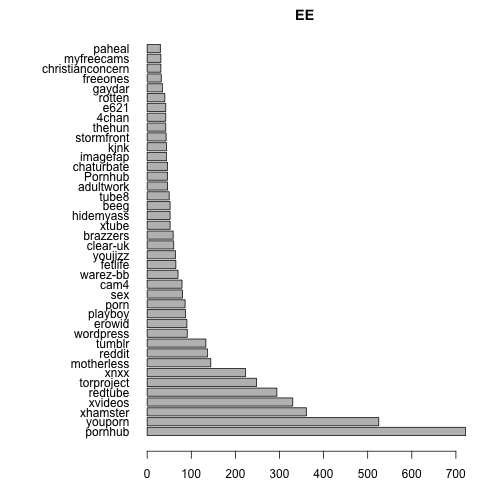
\includegraphics[width=0.49\textwidth]{imgs/EE-blocked-pages-to-date}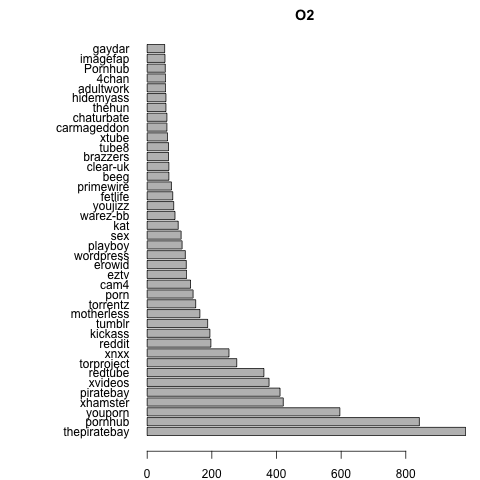
\includegraphics[width=0.49\textwidth]{imgs/O2-blocked-pages-to-date}
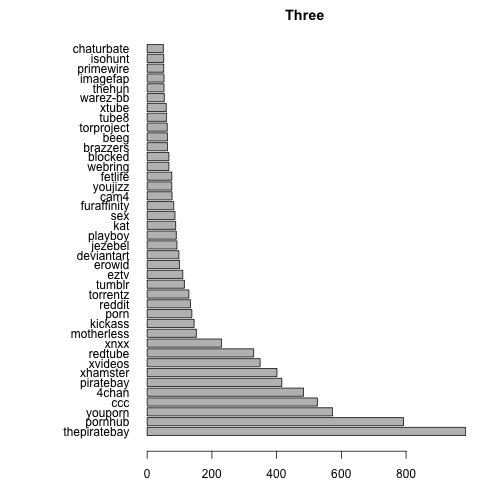
\includegraphics[width=0.49\textwidth]{imgs/Three-blocked-pages-to-date.png}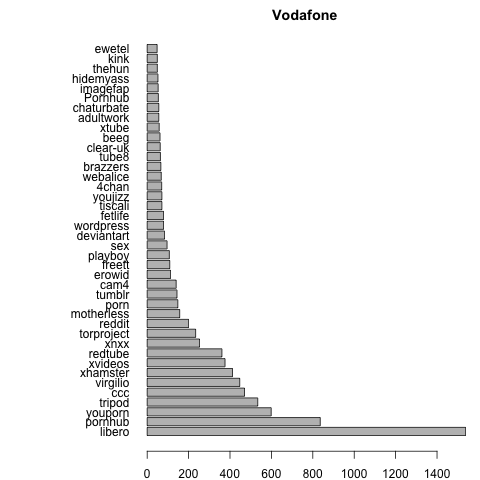
\includegraphics[width=0.49\textwidth]{imgs/Vodafone-blocked-pages-to-date}
\label{fig:mobile-blocked-domains}
\end{figure}

\subsubsection*{Overblocked Sites}
Our macro-level analysis of blocked domains revealed that certain filters were blocked site domains that are not normally associated with adult-content.
To examine further what these sites were, and to find out if they indeed contained adult content, we extracted blocked sites with domains from \url{wordpress}, \url{tumblr}, \url{reddit}, and \url{livejournal}; we now describe \textit{overblocked} sites from each (i.e. sites that should not have been blocked by the filters):

\begin{itemize}
	\item \url{http://garsai.wordpress.com} - Radio documentary site. Blocked by TalkTalk. 
	\item \url{http://toysoldier.wordpress.com} - This site is a support site for men who have been abused. Blocked by Sky and O2.
	\item \url{http://www.heyartist.wordpress.com} - Site promoting art as a support mechanism for enhancing wellbeing. Blocked by Sky.
	\item \url{http://azurelunatic.tumblr.com/post/18654147576/ive-been-forced-to-explain-homosexuality-to-my} - Page explaining why someone is gay. Blocked by Vodafone, O2, TalkTalk, and BT.
	\item \url{http://thusly.tumblr.com} - Personal web blog containing artistic materials and shared music. Blocked by EE, BT, Sky, O2, and Vodafone.
	\item \url{http://reddit.com/r/creepypms} - Subreddit sharing creepy private messages that people have received. Not necessarily adult content, and definitely not pornography. Blocked by EE.
	\item \url{http://community.livejournal.com/asi/} - Anorexia and self-harm support community site. Contains posts from people explaining their afflictions and getting support from other people. Blocked by Sky.
	\item \url{http://urban-decay.livejournal.com} - Photos of urban areas that have fallen into decline. Blocked by Sky, Three, and O2.
	\item \url{http://ercasse-ainince.livejournal.com/30230.html} - Article about films that have been out for a long time. Blocked by Sky.
\end{itemize}

\subsection*{Blocked Site Categories}
Examining the domains of blocked sites allows for an insight into whether sites are being \textit{overblocked}, while our inspection of specific domains' URLs revealed that certain sites and pages were indeed being blocked when they should not have been - based on the ISPs' and MSPs' filter descriptions.
However, manual inspection of the sites from the blocked records, in to understand what content they contain, is not feasible given their large scale (33,297).
Therefore to overcome this issue, we harnessed DMOZ (Directory MOZilla)\footnote{\url{http://www.dmoz.org/}} which is based on the original Open Directory Project.
DMOZ provides a community-created and maintained categorisation system of web sites: users submit URLs of sites and tag the category (from a previously defined hierarchy) that the sites belong to (one category per site).
The submissions are then verified by the community, thereby ensuring that sites are labelled appropriately.

The DMOZ categorisation system uses ODP categories which can extend to several levels within the category taxonomy's hierarchy, therefore we were able to examine the distribution of blocked categories of sites up to a given depth $d$.
This process involved looking up, for each ISP and MSP, the blocked sites' categories and then recording the frequency distribution of the categories.
Below we show the top-40 blocked categories up to a depth of 4 for ISPs (excluding PlusNet from our analysis as this ISP only blocks file sharing platforms) - in Figure \ref{fig:broadband-blocked-categories}.\footnote{N.b. We used a depth of 4 here in order to show how specific the categories can be, while not being too specific. We have also produced the blocked categories for depths of 3, 5 and 6, the plots of which can be found in the github repository - \url{https://github.com/openrightsgroup/cmp-analysis/tree/master/plotting-scripts/plots/per-isp-filter}}
As expected, several adult categories are found within the top-40 covering different sub-trees within the DMOZ taxonomy; however categories of sites appear to the blocked that one would not associate with adult-content (as with the domains above), such as: \url{Recreation/Food/Drink}, \url{Art/Music/Styles}, \url{World/Deutsch/Computers}, etc.
However, as we will show below, several sites are placed within these categories which are, indeed, adult in nature and should be blocked as per the filter settings - i.e. covering topics such as alcohol.

\begin{figure}[h!]
\caption{\csentence{Distributions of blocked level-4 categories for broadband ISPs.}}
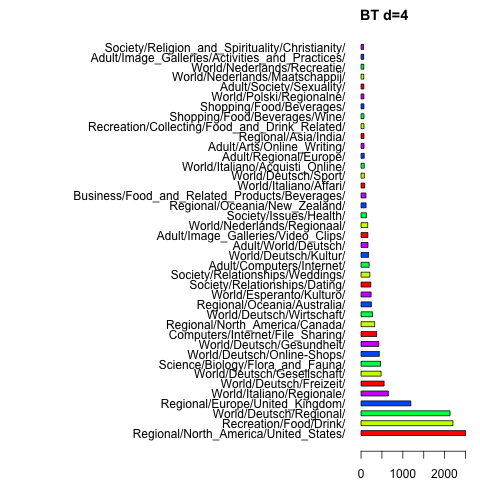
\includegraphics[width=0.49\textwidth]{imgs/BT-d-4-blocked-categories-to-date.png}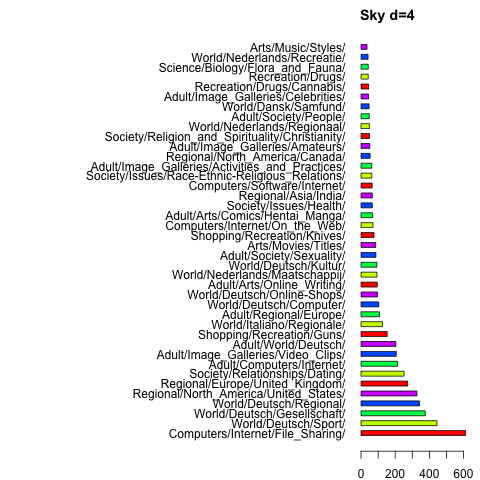
\includegraphics[width=0.49\textwidth]{imgs/Sky-d-4-blocked-categories-to-date.png}
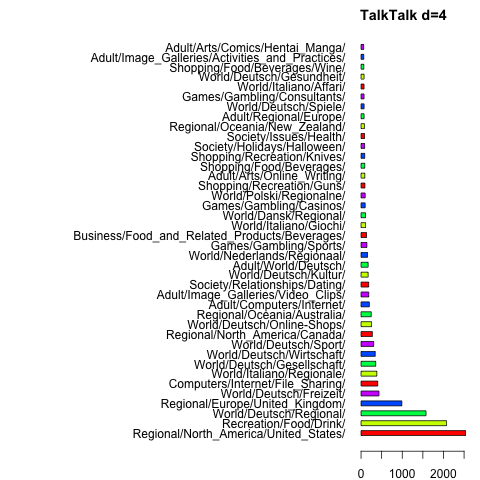
\includegraphics[width=0.49\textwidth]{imgs/TalkTalk-d-4-blocked-categories-to-date.png}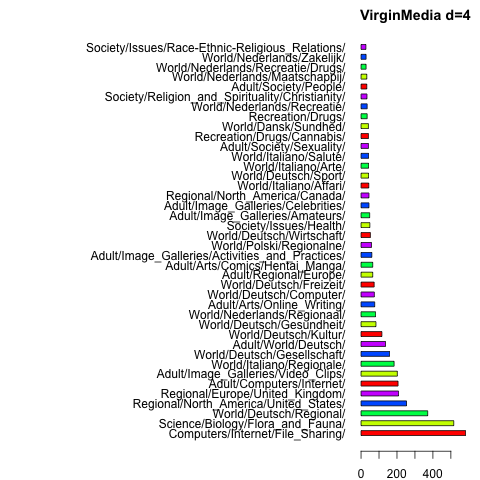
\includegraphics[width=0.49\textwidth]{imgs//VirginMedia-d-4-blocked-categories-to-date.png}
\label{fig:broadband-blocked-categories}
\end{figure}

We found similar distributions of blocked categories for the MSPs as we did for the ISPs - as shown in Figure \ref{fig:mobile-blocked-categories}.

\begin{figure}[h!]
\caption{\csentence{Distributions of blocked level-4 categories for mobile ISPs.}}
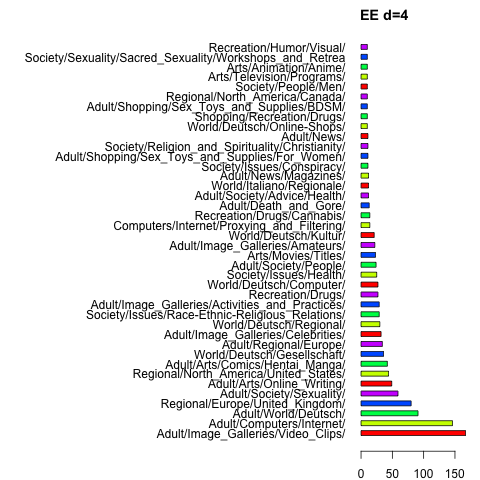
\includegraphics[width=0.49\textwidth]{imgs/EE-d-4-blocked-categories-to-date.png}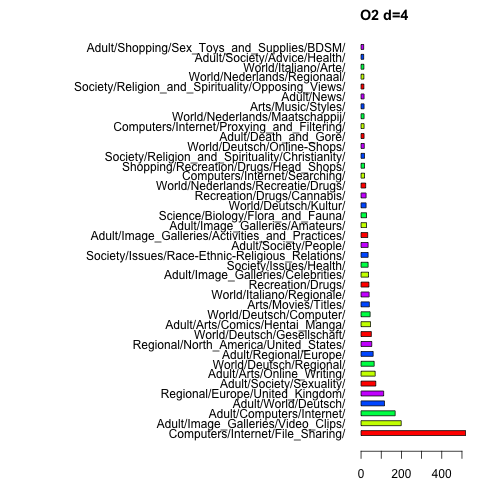
\includegraphics[width=0.49\textwidth]{imgs/O2-d-4-blocked-categories-to-date.png}
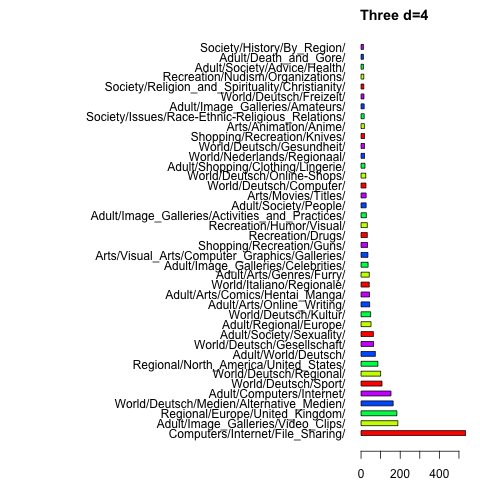
\includegraphics[width=0.49\textwidth]{imgs/Three-d-4-blocked-categories-to-date.png}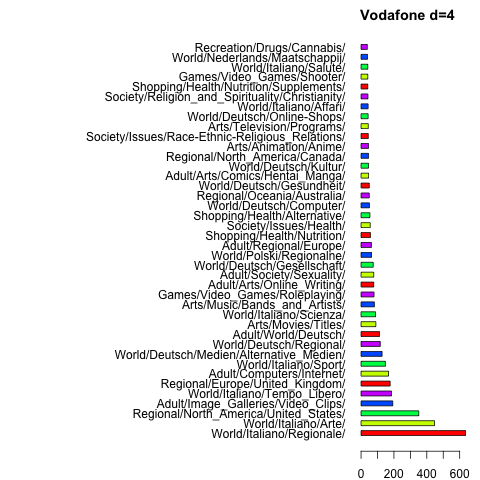
\includegraphics[width=0.49\textwidth]{imgs/Vodafone-d-4-blocked-categories-to-date.png}
\label{fig:mobile-blocked-categories}
\end{figure}


%%%%%% Section
\clearpage
\section*{Gauging Filter Accuracy}
Thus far our inspection of ISPs' and MSPs' filters has been through exploring the domains and categories of blocked sites, and has revealed \textit{qualitative} examples of \textit{overblocking}.
We now turn to answering our first research question: \textit{How can we understand how UK ISP Web Filters function, and how accurate they are?}
To do this we proposed an approach that constructs \textit{Pseudo Classifiers} for each ISP and MSP filter.
These psuedo classifiers are then used to identify what \textit{should} be blocked and what \textit{should not} be blocked, based on the filters' settings' descriptions; in doing so, we can then gauge the \textit{accuracy} of each filter.
We begin this section by explaining how we construct the pseudo classifiers for each filter.

\subsection*{Pseudo-Classifiers for ISP and MSP Filters}
Construction of the pseudo-classifier for each ISP and MSP used the DMOZ categorisation system in conjunction with each filter's documentation to understand what should be blocked and by whom.
In order to aid comprehension of what should be blocked Table \ref{tab:pseudo_classifiers} collates each filter's settings together with the categories of blocked sites.
By default, pornography and obscene and tasteless content (e.g. gore, death, etc.) is blocked across all filters, ISPs all block hate and self-harm sites while MSPs do not, and ISPs vary in which categories of content they block - with TalkTalk being the most strict of all the filters.

\begin{table}[h!]
\caption{Categories that are blocked by each ISP and MSPs' pseudo-classifier according to filter documentation.}
  \begin{tabular}{ l | c c c c | c c c c }
    \hline
	& BT & Sky & TalkTalk & VirginMedia & EE & O2 & Three & Vodafone \\
    \hline
    Pornography & $\times$ & $\times$ & $\times$ & $\times$ & $\times$ & $\times$ & $\times$ & $\times$ \\ 
    Obscene and Tasteless & $\times$ & $\times$ & $\times$ & $\times$ & $\times$ & $\times$ & $\times$ & $\times$ \\
    Hate and Self-harm & $\times$ & $\times$ & $\times$ & $\times$ & \\   
	Drugs & $\times$ & $\times$ & $\times$ & $\times$ & $\times$ \\
	Alcohol & $\times$ & & $\times$ & & $\times$ \\
	Tobacco & $\times$ & & $\times$ & & $\times$ \\	
	Dating & $\times$ & $\times$ & $\times$ & & & & & $\times$ \\
	Social Networking & & $\times$ & $\times$ & & \\
	Gambling & & $\times$ & $\times$ & & & & & $\times$ \\
	File-sharing & & & $\times$ & $\times$ & \\
	Violence & & & $\times$ & & \\
	Gaming & & & $\times$ & & \\
	Malware & & $\times$ & $\times$ & & \\
    \hline
  \end{tabular}
  \label{tab:pseudo_classifiers}
\end{table}

In order to operationalise these categories, we identified equivalent DMOZ categories that sites had been mapped to.
For the DMOZ categories we selected the most \textit{general} category possible, therefore should a site be placed in a sub-category then this would be detected.
For instance, for the category \textit{Tobacco} we used the DMOZ categories \url{Shopping/Tobacco} and \url{Recreation/Tobacco}.
Our approach was to be as conservative as possible here and to ensure that a filter would block any category that we were unsure about - e.g. blocking all sites listed under \url{Computers/Hacking}.
Certain categories of sites were ambiguous and could contain content that should be blocked and content that should not be blocked.
For instance, we found that several alcohol and tobacco related web sites were contained in the \url{World} category, therefore we excluded this category of site completely from our analysis.
Likewise, we also excluded any sites categorised under \url{Computers/Software/Internet/File_Sharing} as this was also found to be ambiguous.
For a full listing of the blocked categories and their DMOZ category mappings please refer to the appendices.


%-Induce a pseudo-classifier for each ISP filter setting:
%--Specify which categories of content should be blocked by certain filter
%--Add table to explain this
%--Coded blocked topics into DMOZ categories to identify what the pseudo classifier should block. 
%--Our approach is to always go as conservative as possible: i.e. if unsure about whether a category should be blocked, then block it.
%--Remove file-sharing for now, as this is assessed on a case-by-case basis and with court orders
%---I.e. blocking all of Computers: Software: Internet: File Sharing would lead to studies on file-sharing being blocked
%--Hence: block everything under Adult
%--Also block everything under Computers/Hacking
%
%VirginMedia: should block...
%--Crime, Violence, and Hate: (Adult)
%--Drugs (Recreation/Drugs/Cannabis + Recreation/Drugs/Psychedelics)
%--File Sharing Sites (Computers/Software/Internet/Clients/File Sharing)
%--Pornography (Adult)
%--Suicide and Self-harm (no category for this in DMOZ)
%
%-BT: should block...
%--pornography (Adult/Image Galleries + Adult/Video Clips)
%--obscene and tasteless (Adult/Death and Gore)
%--hate and self-harm (no DMOZ category)
%--drugs (Recreation/Drugs)
%--alcohol (Recreation/Food/Drink/Drinking + Health/Specific Substances/Alcoholic Beverages)
%--tobacco (Shopping/Tobacco + Recreation/Tobacco)
%--dating (Society/Relationships/Dating, Society/Relationships/Cyber\_Relationships)
%-Sky: should block...
%--malware sites (Computers/Security/Malicious\_Software/Spyware\_and\_Adware)
%--cyber-bullying (no cat on this, generally there are advice pages though)
%--pornography (Adult)
%--suicide and self-harm (no cat)
%--drugs (Recreation/Drugs)
%--dating (Society/Relationships/Dating)
%--social networking (Computers/Internet/On\_the\_Web/Online\_Communities/Social\_Networking, Kids\_and\_Teens/People\_and\_Society/Online Communities)
%--online gaming (Games/Online)
%
%-TalkTalk: should block...
%--dating (Society/Relationships/Dating)
%--drugs (Recreation/Drugs)
%--alcohol (Recreation/Food/Drink/Drinking + Health/Specific Substances/Alcoholic Beverages)
%--tobacco (Shopping/Tobacco + Recreation/Tobacco)
%--File Sharing Sites (Computers/Software/Internet/Clients/File Sharing)
%--Gambling (Gamling)
%--online gaming (Games)
%--Pornography (Adult)
%--social networking (Computers/Internet/On\_the\_Web/Online\_Communities/Social\_Networking, Kids\_and\_Teens/People\_and\_Society/Online Communities)
%--Suicide and Self-Harm (no cat)
%--Weapons and Violence (Adult)
%
%
%
%
%-EE, O2, and Three: should block...
%
%--18 works are for adults and can contain strong issues such as: very strong violence, frequent strong language (e.g. 'f***') and / or very strong language (e.g. ‘c***’), strong portrayals of sexual activity, scenes of sexual violence, strong horror, strong blood and gore, real sex (in some circumstances), discriminatory language and behaviour
%
%-Vodafone: should block...
%--Our content control prevents access to 18-rated content on Vodafone live! (mobile internet) and blocks access to 18-rated websites, un-moderated chat rooms and listed child abuse sites.
%
%
%
%From the DMOZ web site: 
%Generally the Adult category includes sites whose dominant theme is either:
%-To appeal to the prurient interest in sex without any serious literary, artistic, political, or scientific value
%-The depiction or description of nudity, including sexual or excretory activities or organs in a lascivious way
%-The depiction or description of sexually explicit conduct in a lascivious way (e.g. for entertainment purposes)



\subsection*{Judging Filter Accuracy}
Once the pseudo-classifiers were constructed for each filter we could then judge how well each filter performs \textit{overall} before then assessing how accuracy changes over time.
To judge the accuracy of the filters we borrow five measures of performance from machine learning and supervised classification tasks in particular.
In such classification, the goal is to induce a model that can, as accurately as possible, differentiate between classes of objects (e.g. types of customers, predicting rain or not the following day, etc.).
In the context of our analyses we have a similar task: \textit{should a given web site be blocked or not?}
Therefore, we can resolve each filter to handle a set of web sites where we compare each filter's actual labels for the sites (blocked or not) against whether the sites should have been blocked or not.
This can be summarised in the following contingency table:

\begin{table}[h!]
\caption{Contingency table for deriving filters' accuracy measures.}
  \begin{tabular}{ l l | c c | }
 &  & \multicolumn{2}{| c |}{Gold Standard} \\
 & & Block & Not block \\
 \hline
 \multirow{2}{*}{Outcome} & Block & True Positive (TP) & False Positive (FP)  \\
						   & Not block & False Positive (FP) & True Negative (TN) \\
  \end{tabular}
  \label{tab:contingency}
\end{table}

In using the above formulation we can count how many False Positives as the number of URLs that were incorrectly blocked; and False Negatives as the number of URLs that were incorrectly not blocked.
Hence, the former measures the extent to which \textit{overblocking} occurs while the latter gauges the magnitude of \textit{underblocking}.
In order to gauge the relative performance of the filters, we use the following accuracy measures: (i) Precision, gauges the proportion of URLs labelled as \textit{blocks} that were correct; (ii) Recall, to measure the proportion of blocked URLs that should have been detected; and (iii) F-measure (F1) as the harmonic mean between precision and recall.
These accuracy measures are defined explicitly, using the contingency table defined in Table \ref{tab:contingency}, as follows:
	
\begin{equation}
precision = \frac{\vert TP \vert}{\vert TP \vert  + \vert FP \vert}, \quad recall = \frac{\vert TP \vert }{ \vert TP \vert  + \vert FN \vert}, \quad F1 = \frac{ 2 \times precision \times recall }{precision + recall} 
\end{equation}
	
We also define two additional accuracy measures as follows: the first of the False Positive Rate (FPR) which measures the proportion of false positives that are produced by the filter, defined as:

\begin{equation}
FPR = \frac{\vert FP \vert}{ \vert FP \vert + \vert TN \vert}
\end{equation}

Hence, if the magnitude of $TN$ increases and $FP$ decreases then the classifier produces fewer overblocks.
For precision, recall, F1 and FPR all values are within the closed interval $[0,1]$ with a value of 1 indicating perfect performance for precision, recall, and F1 - and the opposite for FPR (as we wish to minimise this value).

We also included the \textit{Matthews Correlation Coefficient} as our fifth and final accuracy measure.
This measure produces a value in the closed interval $[-1, 1]$ with: $0$ indicating that the filter matches a random guesser's accuracy, $1$ indicating perfect performance far superior to a random guesser, and a value of $-1$ indicating that all outcomes of the filter were incorrect.

\subsubsection*{Parallelised Computation}
As we were dealing with 8 different filters, and their pseudo-classifiers, and had to process 6 million records - which are growing in size daily as the probes collect more data - we constructed a parallel-processing framework to compute the accuracy measures for each filter.
This framework was written using the Apache Spark stack and utilised HDFS from the Apache Hadoop stack - the Python code can be found online in the Github repository of the project.\footnote{\url{https://github.com/openrightsgroup/cmp-analysis}}
Computation follows a pipeline approach as follows:
\begin{enumerate}
	\item Clean and load data into HDFS. The blocked.org.uk export file containing all requests is cleaned to reduce duplicate records and then loaded into HDFS.
	The DMOZ category files are also loaded into HDFS.
	\item Load DMOZ category map into cluster memory. The DMOZ category file is processed using a map-reduce job thereby producing \texttt{(key, value)} pairs where the keys are URLs and the values are the DMOZ category - one URL has one category. 
	We actually load the non-adult category map and the adult category map separately - as DMOZ provides different files for each - and then perform \texttt{union} operation to join the maps.
	This joined map is then broadcast to the cluster so that all nodes can access the map from memory.
	\item Compute contingency tables per ISP and MSP. A second map-reduce job is run to produce (key, value) pairs from the cleaned request export file in HDFS.
	Keys here are the ISP and MSP names (e.g. BT, O2, etc.) and values are contingency table objects.
	The \textit{map}-stage functions by reading in one line from the export file and then checking if the request is a block or not and for which ISP it pertains to, a new contingency table is then produced for the (key, value) pair.
	The \textit{reduce}-stage then combines all of the contingency tables together for the given filter.
	\item Accuracy computation. After the final map-reduce job is complete, the above accuracy measures are then computed for each ISP and MSP based on the combined contingency tables.
\end{enumerate}

The above approach is an effective way of quickly processing the requests file and gauging filter accuracy.
As we will explain below, this framework also allows for time-series computation of filter accuracy to be performed.


\subsubsection*{General Accuracy}

%% Original results without assessing for polysemic categories
%\begin{table}[h!]
%\caption{Accuracy levels of ISP and Mobile Providers' Web Filters derived using the DMOZ categories that should have been blocked by each filter and the categories of URLs that were actually blocked.}
%  \begin{tabular}{ l c c c c c c}
%    \hline
%     & Precision & Recall & FPR & MCC & F1 \\
%    \hline
%	BT & 0.032 & 0.613 & 0.012 & 0.138 & 0.061 \\
%    Sky & 0.088 & 0.370 & 0.003 & 0.179 & 0.142 \\
%    TalkTalk & 0.078  & 0.073 & 0.009 & 0.066 & 0.075 \\
%	VirginMedia & 0.050 & 0.508 & 0.003 & 0.159 & 0.091 \\
%	\hline    
%	EE & 0.189 & 0.635 & 0.002 & 0.346 & 0.291 \\
%	O2 & 0.136 & 0.697 & 0.002 & 0.307 & 0.227 \\
%	Three & 0.108 & 0.631 & 0.004 & 0.260 & 0.185 \\
%	Vodafone & 0.044 & 0.564 & 0.004 & 0.156 & 0.081 \\
%    \hline
%  \end{tabular}
%\end{table}
%
%% Updated results (21st May 2015). Shows large degradation in accuracy. After altering category checking procedure
%%BT: tp = 634.0 | tn = 1543183.0 | fp = 19168.0 | fn = 400.0 | prec = 0.032 | rec = 0.613 | FPR = 0.012 | mcc = 0.138 | F1 = 0.061
%%Sky: tp = 526.0 | tn = 1566677.0 | fp = 5442.0 | fn = 895.0 | prec = 0.088 | rec = 0.370 | FPR = 0.003 | mcc = 0.179 | F1 = 0.142
%%TalkTalk: tp = 1218.0 | tn = 1542758.0 | fp = 14409.0 | fn = 15514.0 | prec = 0.078  | rec = 0.073 | FPR = 0.009 | mcc = 0.066 | F1 = 0.075
%%VirginMedia: tp = 266.0 | tn = 1568395.0 | fp = 5036.0 | fn = 258.0 | prec = 0.0502  | rec = 0.508 | FPR = 0.003 | mcc = 0.159 | F1 = 0.091
%%EE: tp = 219.0 | tn = 472432.0 | fp = 939.0 | fn = 126.0 | prec = 0.189 | rec = 0.635 | FPR = 0.002 | mcc = 0.346 | F1 = 0.291
%%O2: tp = 230.0 | tn = 876122.0 | fp = 1462.0 | fn = 100.0 | prec = 0.136 | rec = 0.697 | FPR = 0.002 | mcc = 0.307 | F1 = 0.227
%%Three: tp = 236.0 | tn = 491864.0 | fp = 1941.0 | fn = 138.0 | prec = 0.108 | rec = 0.631 | FPR = 0.004 | mcc = 0.260 | F1 = 0.185
%%Vodafone: tp = 254.0 | tn = 1482343.0 | fp = 5560.0 | fn = 196.0 | prec = 0.044 | rec = 0.564 | FPR = 0.004 | mcc = 0.156 | F1 = 0.081
%
%\begin{table}[h!]
%\caption{Accuracy levels after filtering out sites from the World category subtree.}
%  \begin{tabular}{ l c c c c c c}
%    \hline
%     & Precision & Recall & FPR & MCC & F1 \\
%    \hline
%	BT & 0.066 & 0.612 & 0.010 & 0.198 & 0.119 \\
%    Sky & 0.163 & 0.372 & 0.003 & 0.245 & 0.227 \\
%    TalkTalk & 0.145 & 0.072 & 0.008 & 0.091 & 0.097 \\
%	VirginMedia & 0.112 & 0.512 & 0.002 & 0.239 & 0.184 \\
%	\hline    
%	EE & 0.281 & 0.637 & 0.002 & 0.422 & 0.390 \\
%	O2 & 0.218 & 0.699 & 0.002 & 0.390 & 0.333 \\
%	Three & 0.184 & 0.633 & 0.004 & 0.340 & 0.285 \\
%	Vodafone & 0.083 & 0.568 & 0.003 & 0.216 & 0.144 \\
%    \hline
%  \end{tabular}
%\end{table}
%
%
%% Updated results (29th May 2015). After altering the world category filter
%%BT: tp = 627.0 | tn = 867824.0 | fp = 8919.0 | fn = 398.0 | prec = 0.066 | rec = 0.612 | FPR = 0.010 | mcc = 0.198 | F1 = 0.119
%%Sky: tp = 520.0 | tn = 879512.0 | fp = 2663.0 | fn = 876.0 | prec = 0.163 | rec = 0.372 | FPR = 0.003 | mcc = 0.245 | F1 = 0.227
%%TalkTalk: tp = 1201.0 | tn = 860146.0 | fp = 7065.0 | fn = 15375.0 | prec = 0.145 | rec = 0.072 | FPR = 0.008 | mcc = 0.091 | F1 = 0.097
%%VirginMedia: tp = 266.0 | tn = 881118.0 | fp = 2105.0 | fn = 254.0 | prec = 0.112 | rec = 0.512 | FPR = 0.002 | mcc = 0.239 | F1 = 0.184
%%EE: tp = 219.0 | tn = 269566.0 | fp = 561.0 | fn = 125.0 | prec = 0.281 | rec = 0.637 | FPR = 0.002 | mcc = 0.422 | F1 = 0.390
%%O2: tp = 230.0 | tn = 494277.0 | fp = 823.0 | fn = 99.0 | prec = 0.218 | rec = 0.699 | FPR = 0.002 | mcc = 0.390 | F1 = 0.333
%%Three: tp = 236.0 | tn = 280598.0 | fp = 1046.0 | fn = 137.0 | prec = 0.184 | rec = 0.633 | FPR = 0.004 | mcc = 0.340 | F1 = 0.285
%%Vodafone: tp = 254.0 | tn = 832797.0 | fp = 2819.0 | fn = 193.0 | prec = 0.083 | rec = 0.568 | FPR = 0.003 | mcc = 0.216 | F1 = 0.144
%
%\begin{table}[h!]
%\caption{Accuracy levels after filtering out sites from the World category subtree and controlling for breweries and other alcohol related sites.}
%  \begin{tabular}{ l c c c c c c}
%    \hline
%     & Precision & Recall & FPR & MCC & F1 \\
%    \hline
%	BT & 0.335 & 0.726 & 0.007 & 0.490 & 0.459 \\
%    Sky & 0.163 & 0.372 & 0.003 & 0.245 & 0.227 \\
%    TalkTalk & 0.422 & 0.176 & 0.006 & 0.262 & 0.248 \\
%	VirginMedia & 0.112 & 0.512 & 0.002 & 0.239 & 0.184 \\
%	\hline    
%	EE & 0.281 & 0.637 & 0.002 & 0.422 & 0.390 \\
%	O2 & 0.218 & 0.699 & 0.002 & 0.390 & 0.333 \\
%	Three & 0.184 & 0.633 & 0.004 & 0.340 & 0.285 \\
%	Vodafone & 0.083 & 0.568 & 0.003 & 0.216 & 0.144 \\
%    \hline
%  \end{tabular}
%\end{table}

% Updated results (29th May 2015). After fixing the alcohol sites
%BT: tp = 3202.0 | tn = 867015.0 | fp = 6344.0 | fn = 1207.0 | prec = 0.335 | rec = 0.726 | FPR = 0.007 | mcc = 0.490 | F1 = 0.459
%Sky: tp = 520.0 | tn = 879512.0 | fp = 2663.0 | fn = 876.0 | prec = 0.163 | rec = 0.372 | FPR = 0.003 | mcc = 0.245 | F1 = 0.227
%TalkTalk: tp = 3485.0 | tn = 859202.0 | fp = 4781.0 | fn = 16319.0 | prec = 0.422 | rec = 0.176 | FPR = 0.006 | mcc = 0.262 | F1 = 0.248
%VirginMedia: tp = 266.0 | tn = 881118.0 | fp = 2105.0 | fn = 254.0 | prec = 0.112 | rec = 0.512 | FPR = 0.002 | mcc = 0.239 | F1 = 0.184
%EE: tp = 219.0 | tn = 269566.0 | fp = 561.0 | fn = 125.0 | prec = 0.281 | rec = 0.637 | FPR = 0.002 | mcc = 0.422 | F1 = 0.390
%O2: tp = 230.0 | tn = 494277.0 | fp = 823.0 | fn = 99.0 | prec = 0.218 | rec = 0.699 | FPR = 0.002 | mcc = 0.390 | F1 = 0.333
%Three: tp = 236.0 | tn = 280598.0 | fp = 1046.0 | fn = 137.0 | prec = 0.184 | rec = 0.633 | FPR = 0.004 | mcc = 0.340 | F1 = 0.285
%Vodafone: tp = 254.0 | tn = 832797.0 | fp = 2819.0 | fn = 193.0 | prec = 0.083 | rec = 0.568 | FPR = 0.003 | mcc = 0.216 | F1 = 0.144

From the computational framework, we were able to compute the accuracy of each filter as shown in Table \ref{tab:accuracy}.

\begin{table}[h!]
\caption{Accuracy levels of the various ISPs' and MSPs' filters across the five measures.}
  \begin{tabular}{ l c c c c c c}
    \hline
     & Precision & Recall & FPR & MCC & F1 \\
    \hline
	BT & 0.418 & 0.619 & 0.006 & 0.505 & 0.499 \\
    Sky & 0.191 & 0.236 & 0.003 & 0.210 & 0.211 \\
    TalkTalk & 0.483 & 0.183 & 0.005 & 0.287 & 0.266 \\
	VirginMedia & 0.112 & 0.512 & 0.002 & 0.239 & 0.184 \\
	\hline    
	EE & 0.281 & 0.637 & 0.002 & 0.422 & 0.390 \\
	O2 & 0.218 & 0.699 & 0.002 & 0.390 & 0.333 \\
	Three & 0.184 & 0.633 & 0.004 & 0.340 & 0.285 \\
	Vodafone & 0.083 & 0.568 & 0.003 & 0.216 & 0.144 \\
    \hline
  \end{tabular}
  \label{tab:accuracy}
\end{table}




Compare results to that of \cite{stark2007effectiveness}

%BT: tp = 3995.0 | tn = 865766.0 | fp = 5551.0 | fn = 2456.0 | prec = 0.418 | rec = 0.619 | FPR = 0.006 | mcc = 0.505 | F1 = 0.499
%Sky: tp = 607.0 | tn = 878427.0 | fp = 2576.0 | fn = 1961.0 | prec = 0.191 | rec = 0.236 | FPR = 0.003 | mcc = 0.210 | F1 = 0.211
%TalkTalk: tp = 3994.0 | tn = 857742.0 | fp = 4272.0 | fn = 17779.0 | prec = 0.483 | rec = 0.183 | FPR = 0.005 | mcc = 0.287 | F1 = 0.266
%VirginMedia: tp = 266.0 | tn = 881118.0 | fp = 2105.0 | fn = 254.0 | prec = 0.112 | rec = 0.512 | FPR = 0.002 | mcc = 0.239 | F1 = 0.184

%EE: tp = 219.0 | tn = 269566.0 | fp = 561.0 | fn = 125.0 | prec = 0.281 | rec = 0.637 | FPR = 0.002 | mcc = 0.422 | F1 = 0.390
%O2: tp = 230.0 | tn = 494277.0 | fp = 823.0 | fn = 99.0 | prec = 0.218 | rec = 0.699 | FPR = 0.002 | mcc = 0.390 | F1 = 0.333
%Three: tp = 236.0 | tn = 280598.0 | fp = 1046.0 | fn = 137.0 | prec = 0.184 | rec = 0.633 | FPR = 0.004 | mcc = 0.340 | F1 = 0.285
%Vodafone: tp = 254.0 | tn = 832797.0 | fp = 2819.0 | fn = 193.0 | prec = 0.083 | rec = 0.568 | FPR = 0.003 | mcc = 0.216 | F1 = 0.144


%%%% Results using keyword checks for EE, Vodafone and Three
%%%% Boost in precision, yet large reduction in recall due to large increase in false negatives
%BT: tp = 3995.0 | tn = 865766.0 | fp = 5551.0 | fn = 2456.0 | prec = 0.418 | rec = 0.619 | FPR = 0.006 | mcc = 0.505 | F1 = 0.499
%Sky: tp = 607.0 | tn = 878427.0 | fp = 2576.0 | fn = 1961.0 | prec = 0.191 | rec = 0.236 | FPR = 0.003 | mcc = 0.210 | F1 = 0.211
%TalkTalk: tp = 3994.0 | tn = 857742.0 | fp = 4272.0 | fn = 17779.0 | prec = 0.483 | rec = 0.183 | FPR = 0.005 | mcc = 0.287 | F1 = 0.266
%VirginMedia: tp = 266.0 | tn = 881118.0 | fp = 2105.0 | fn = 254.0 | prec = 0.112 | rec = 0.512 | FPR = 0.002 | mcc = 0.239 | F1 = 0.184

%EE: tp = 257.0 | tn = 268361.0 | fp = 523.0 | fn = 1330.0 | prec = 0.329 | rec = 0.162 | FPR = 0.002 | mcc = 0.228 | F1 = 0.217
%O2: tp = 230.0 | tn = 494229.0 | fp = 823.0 | fn = 147.0 | prec = 0.218 | rec = 0.610 | FPR = 0.002 | mcc = 0.364 | F1 = 0.322
%Three: tp = 236.0 | tn = 280573.0 | fp = 1046.0 | fn = 162.0 | prec = 0.184 | rec = 0.593 | FPR = 0.004 | mcc = 0.329 | F1 = 0.281
%Vodafone: tp = 285.0 | tn = 831654.0 | fp = 2788.0 | fn = 1336.0 | prec = 0.093 | rec = 0.176 | FPR = 0.003 | mcc = 0.125 | F1 = 0.121



Qualitative Examples of Blocks:
-BT Block: http://www.lgbtquitsmoking.com/ (site to help people stop smoking).

BT seem to be blocking tattoo web sites too:

We have uploaded the collection of sites which are false positives and false negatives to the github repo.\footnote{\url{https://github.com/openrightsgroup/cmp-analysis/tree/master/data/output}}


\subsubsection*{Accuracy over Time}
How has accuracy evolved over time?
--Discrete time analysis of the accuracy levels - use weekly bins (Bayesian model?) Can we forecast accuracy?


\begin{figure}[h!]
\caption{\csentence{Accuracy of Broadband ISPs' filters over time}. ARIMA(0,0,5) plot of the accuracy measures: precision, recall, f-measure (F1), false positive rate (FPR), and the Matthews' Correlation Coefficient. Weeks are from the start of the ISP-specific filter logging period.}
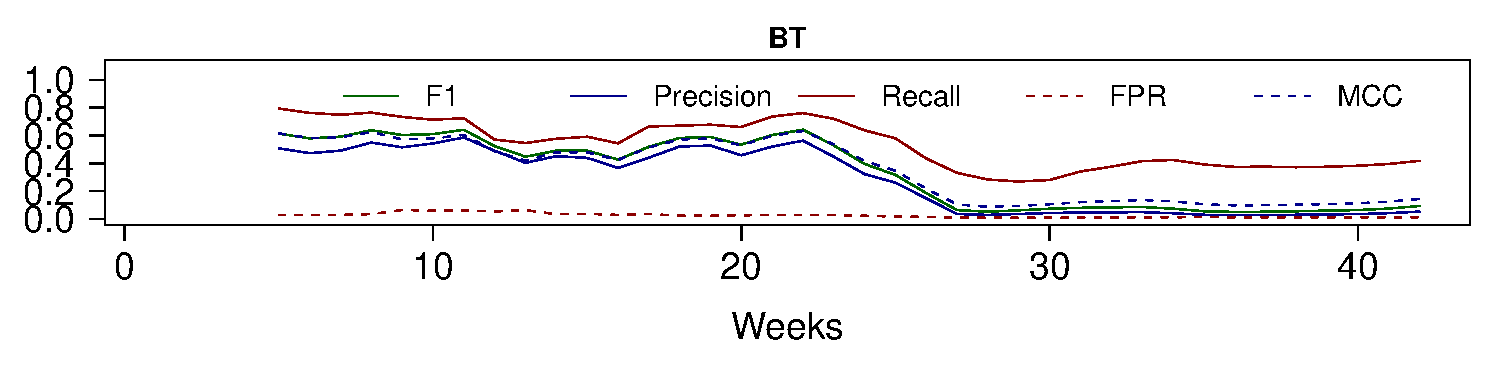
\includegraphics[width=0.9\textwidth]{imgs/BT-ts-accuracy}
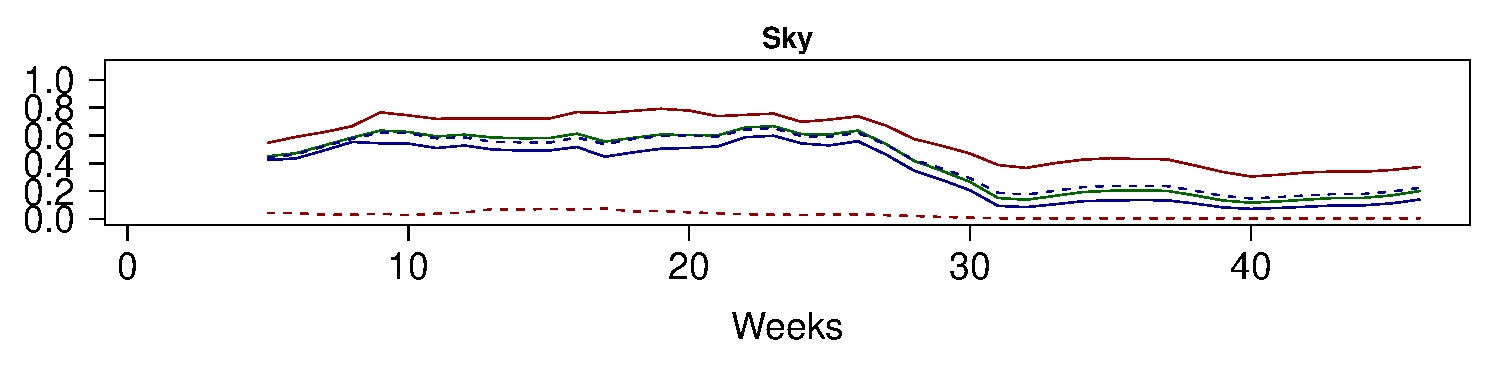
\includegraphics[width=0.9\textwidth]{imgs/Sky-ts-accuracy}
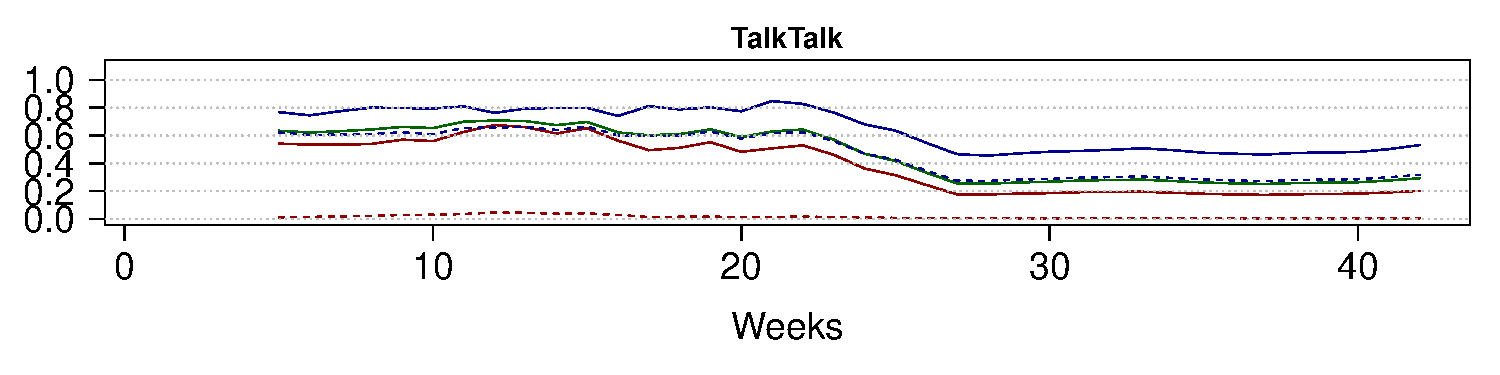
\includegraphics[width=0.9\textwidth]{imgs/TalkTalk-ts-accuracy}
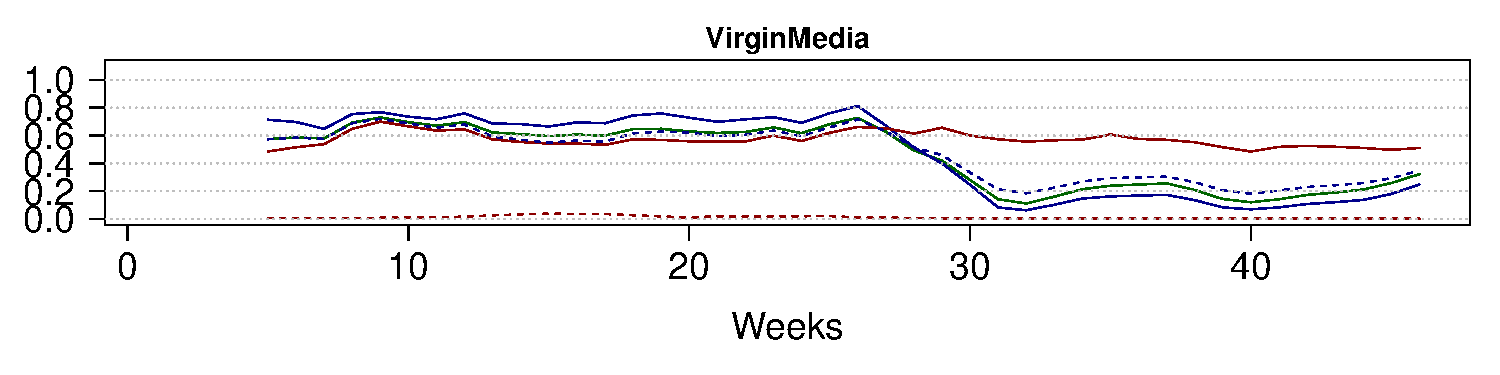
\includegraphics[width=0.9\textwidth]{imgs/VirginMedia-ts-accuracy}
\label{fig:broadband-accuracy-ts}
\end{figure}

\begin{figure}[h!]
\caption{\csentence{Accuracy of Mobile ISPs' filters over time}. ARIMA(0,0,5) plot of the accuracy measures: precision, recall, f-measure (F1), false positive rate (FPR), and the Matthews' Correlation Coefficient. Weeks are from the start of the ISP-specific filter logging period.}
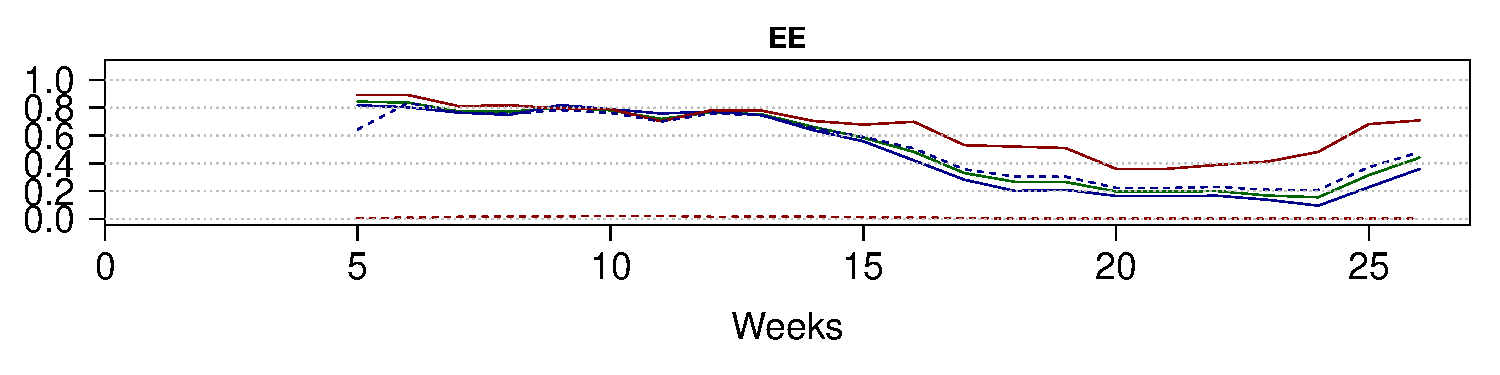
\includegraphics[width=0.9\textwidth]{imgs/EE-ts-accuracy}
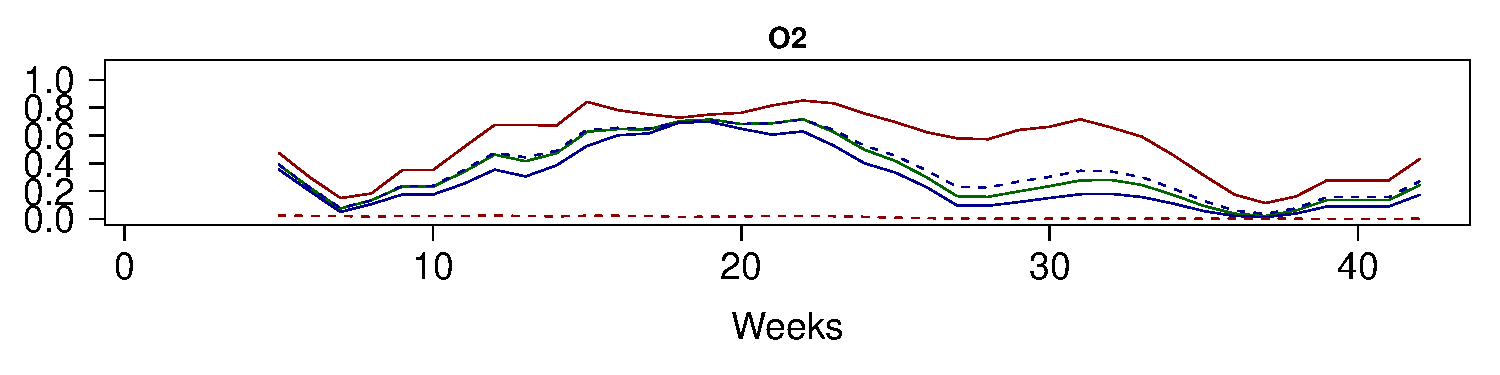
\includegraphics[width=0.9\textwidth]{imgs/O2-ts-accuracy}
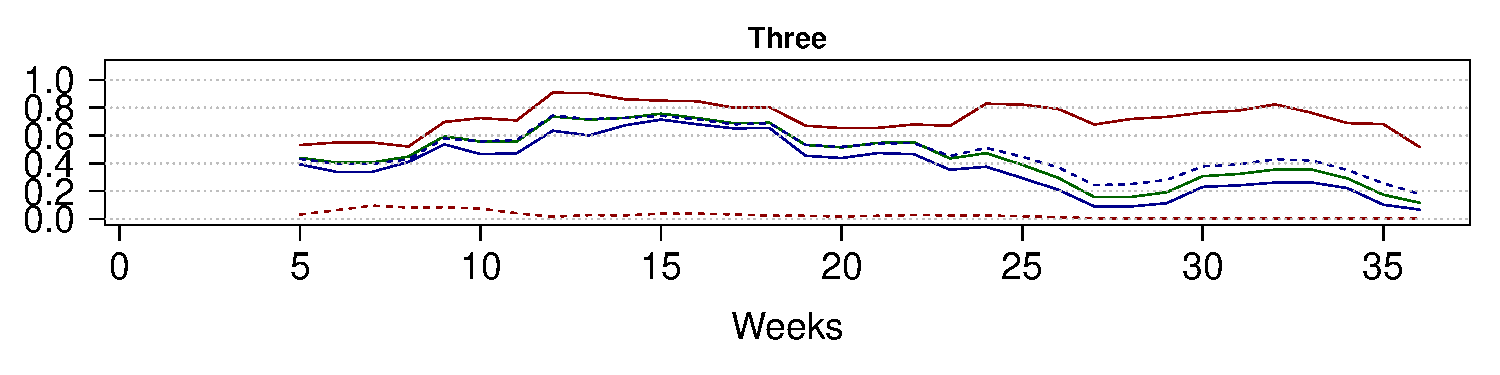
\includegraphics[width=0.9\textwidth]{imgs/Three-ts-accuracy}
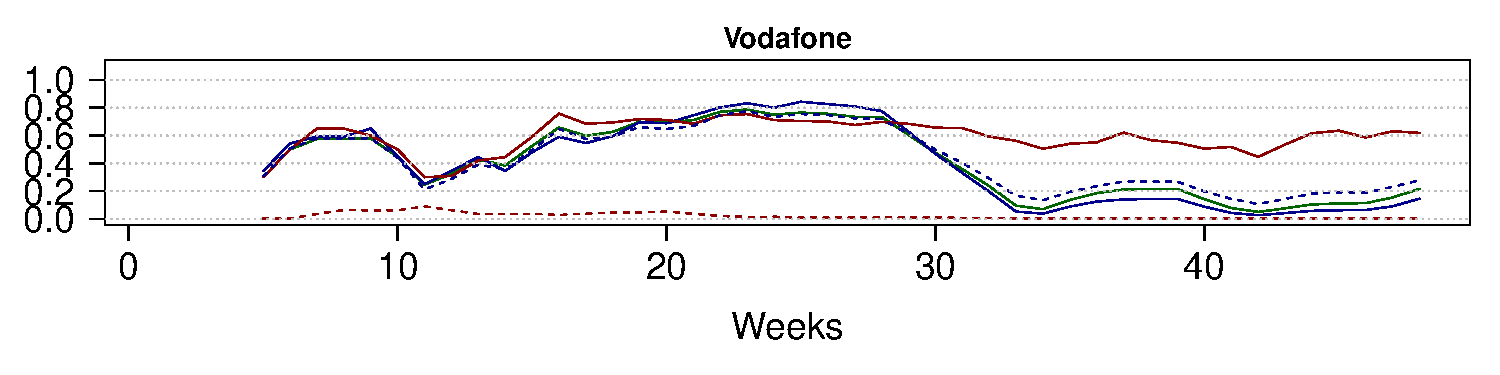
\includegraphics[width=0.9\textwidth]{imgs/Vodafone-ts-accuracy}
\label{fig:mobile-accuracy-ts}
\end{figure}
\clearpage






%%%%%% Section
\section*{Time to Correction}
-Report on how long it takes each ISP to fix their blocked content
-Show the delta distribution of each provider
--Fit a distribution to the delta-function: Poisson?

\begin{figure}[h!]
\caption{\csentence{Time to unblock ($\Delta$) distribution of each Broadband and Mobile ISP in hours}.}
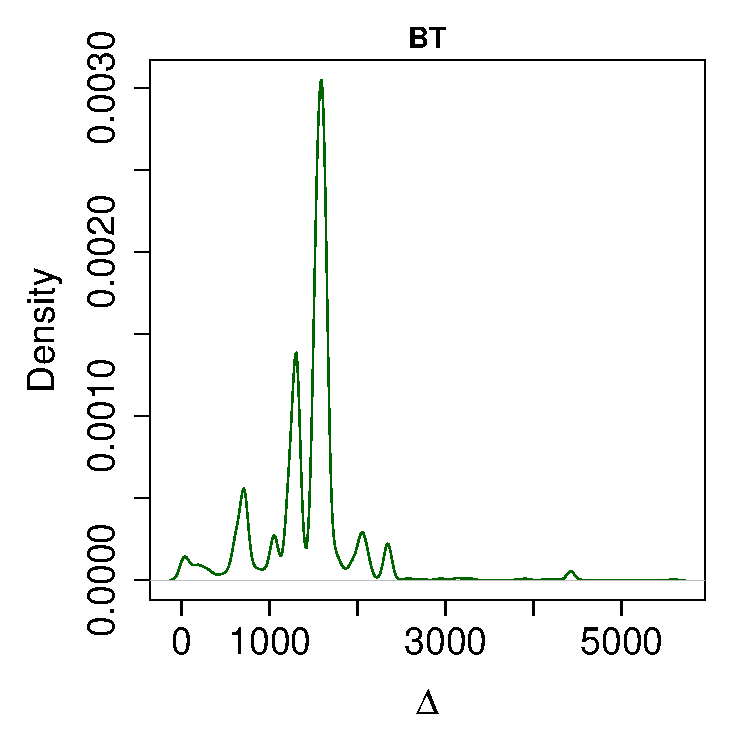
\includegraphics[width=0.2249\textwidth]{imgs/BT-unblock-dist}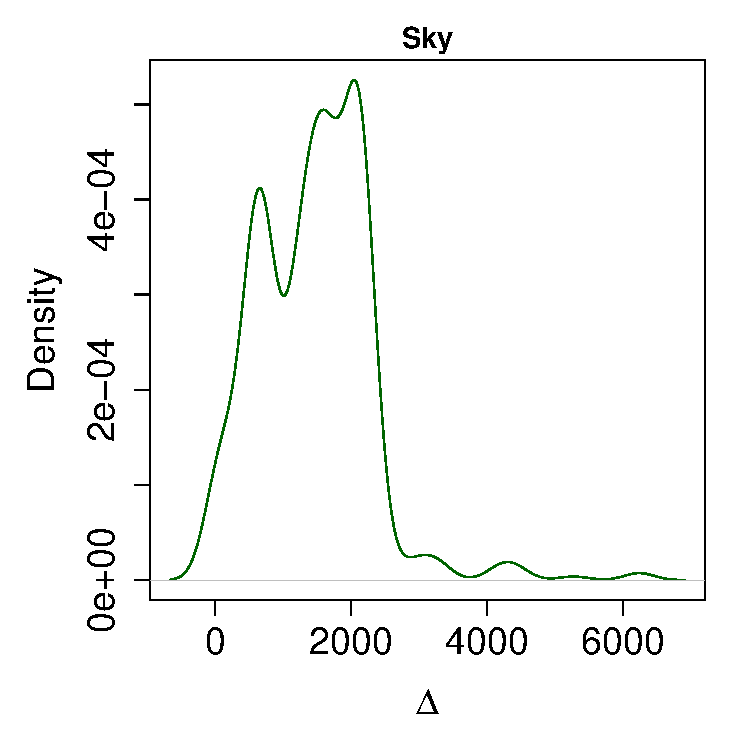
\includegraphics[width=0.2249\textwidth]{imgs/Sky-unblock-dist}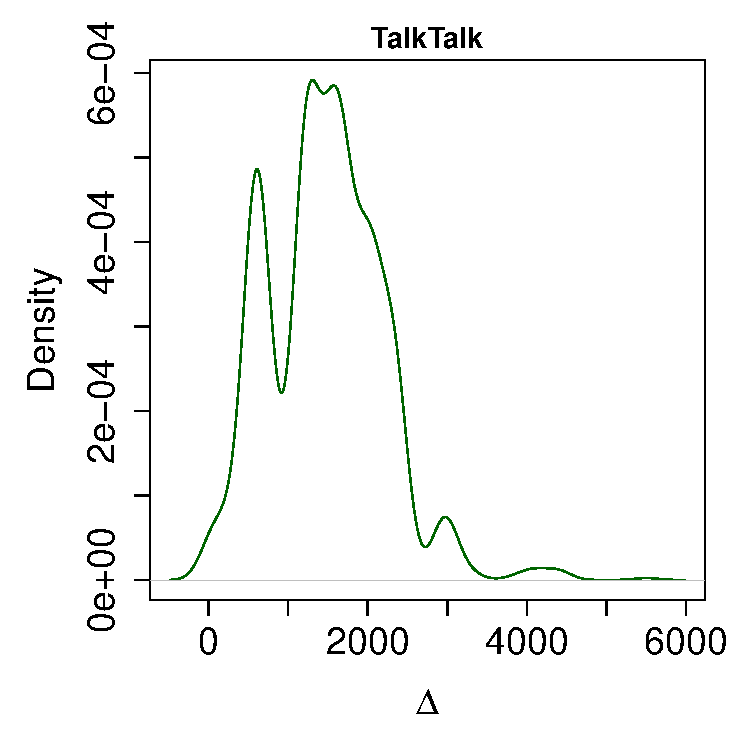
\includegraphics[width=0.2249\textwidth]{imgs/TalkTalk-unblock-dist}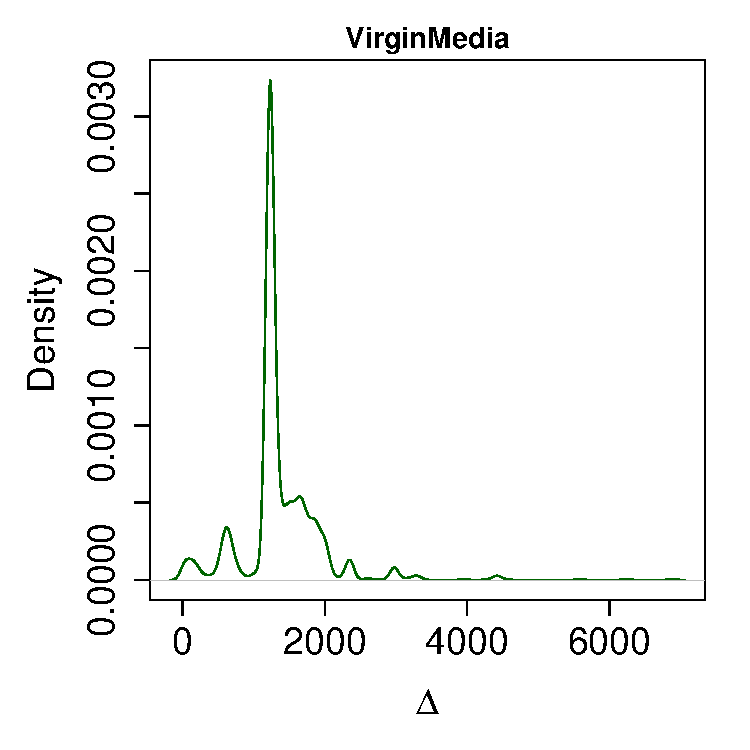
\includegraphics[width=0.2249\textwidth]{imgs/VirginMedia-unblock-dist}

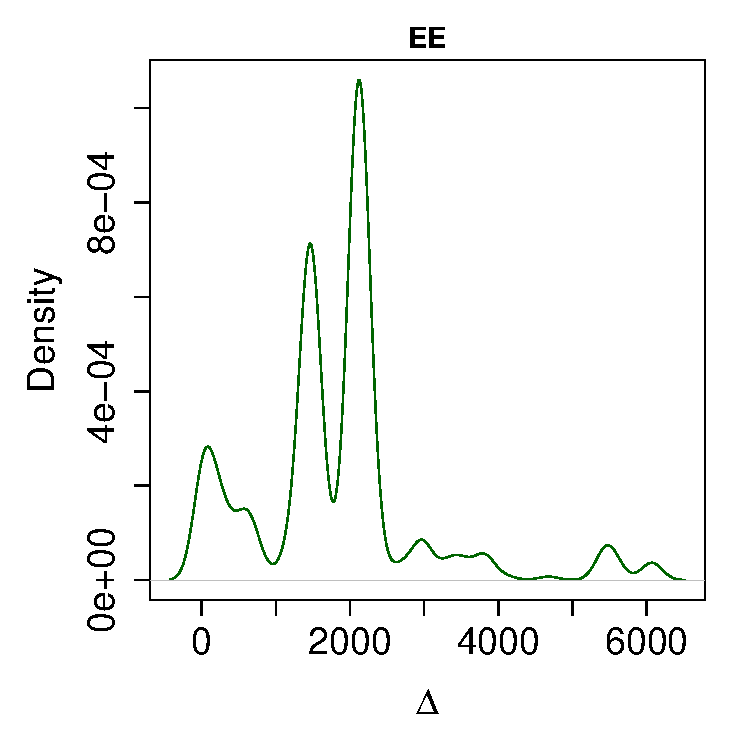
\includegraphics[width=0.2249\textwidth]{imgs/EE-unblock-dist}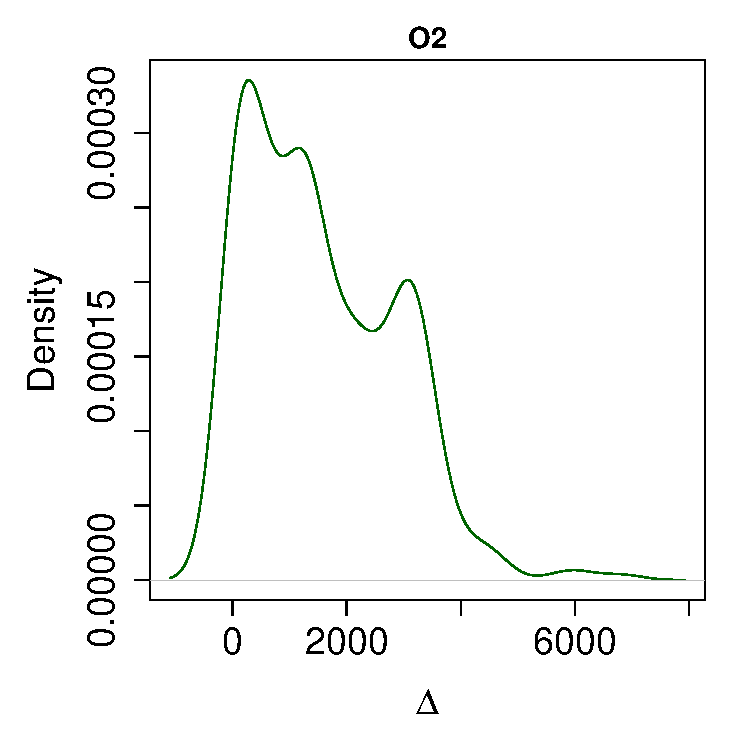
\includegraphics[width=0.2249\textwidth]{imgs/O2-unblock-dist}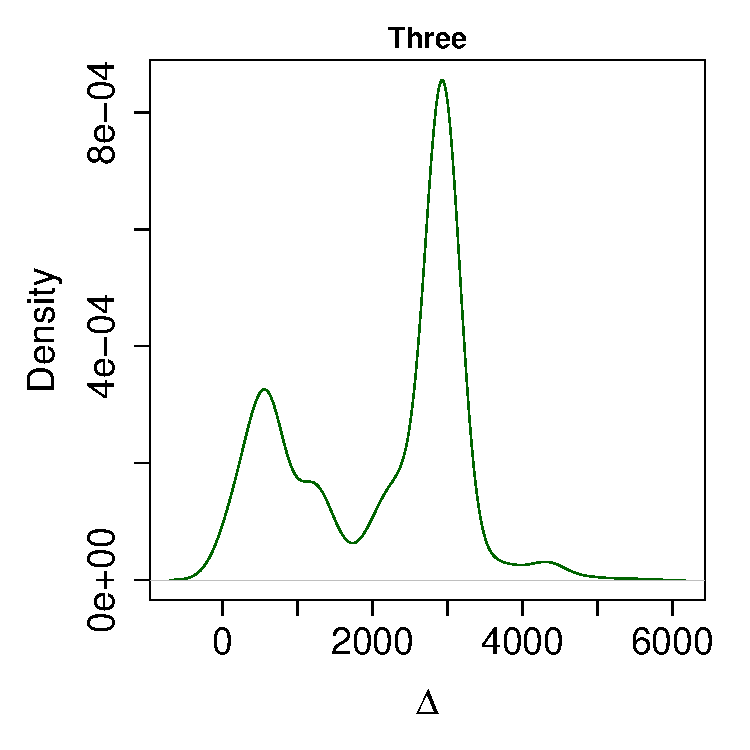
\includegraphics[width=0.2249\textwidth]{imgs/Three-unblock-dist}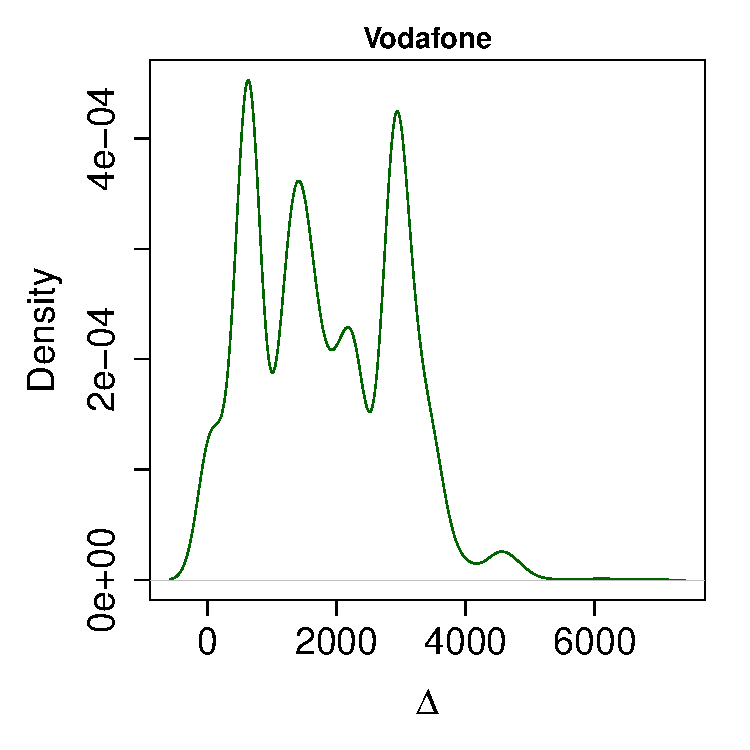
\includegraphics[width=0.2249\textwidth]{imgs/Vodafone-unblock-dist}

\label{fig:isps-unblock-dist}
\end{figure}



%%%%%% Section
\section*{Study Limitations}


\subsection*{Measurement of Blocks}
-Defend the approach of analysing which requests were fulfilled - this can contain duplicate URLs (some of which were blocked, and some of which were not)
--This can lead to repeated URLs in the lists of false/true positives and negatives
--We counteract this by using sets to restrict each URL to one occurrence per set

-Explain possible limitations with the actual probe system itself.


\subsection*{Limitations of Pseudo-Classifiers}
Limitations of this approach:
-Relies on the classification of sites within DMOZ as being correct
-Coverage of the DMOZ categories - as this is manually curated we only cover a \% of the URLs in total that have been aligned with categories

-Use of DMOZ categories is not without errors:
--E.g. the URL http://www.vin-gastronomie.com/ is not classed as should be blocked in the gold standard as its category is ''World: Francais: Regional: Europe: France: Regions: Haute-Normandie: Eure: Commerce et economie: Gastronomie et alimentation', however the page describes wine brands

-Potential improvements:
--Classifying content of the page to mine topics discussed therein - i.e. basic semantic analysis of the content
--Filtering out categories of sites which may introduce noise into the results, and not counting them at all (e.g. those related to gastronomy).


\section*{Findings and Implications}


\section*{Conclusions and Future Work}





\begin{backmatter}

\section*{Competing interests}
  The authors declare that they have no competing interests.

\section*{Acknowledgements}
Open Rights Group for providing the data and engineering the solution

% if your bibliography is in bibtex format, use those commands:
\bibliographystyle{bmc-mathphys} % Style BST file
\bibliography{ORG-Filters-Paper}      % Bibliography file (usually '*.bib' )

\section*{Appendix 1: DMOZ Block Categories}
\label{app:cats}
In order to operationalise the blocked categories we identified equivalent DMOZ categories.
This allowed each filter to have a pseudo-classifier constructed which contained the categories of sites that should be blocked upon request.
These DMOZ categories were as follows:

\begin{itemize}
	\item Adult and Obscene and Tasteless: \url{Adult}
	\item Hate and Self-harm: No category
	\item Drugs: \url{Recreation/Drugs}
	\item Alcohol: \texttt{Recreation/Food/Drink/Drinking, Recreation/Food/Drink/Mead, Recreation/Food/Drink/Wine, Recreation/Food/Drink/Beer, Recreation/Food/Drink/Alcopops, Recreation/Food/Drink/Cider, Recreation/Food/Drink/Cocktails, Recreation/Food/Drink/Liquor, Recreation/Food/Drink/Sake, Health/Specific Substances/Alcoholic Beverages}
	\item Tobacco: \texttt{Shopping/Tobacco, Recreation/Tobacco}
	\item Dating: \url{Society/Relationships/Dating, Society/Relationships/Cyber_Relationships, Regional/Europe/United Kingdom/Society_and_Culture/Gay,_Lesbian,_and_Bisexual/Relationships}
	\item Social Networking: \url{Computers/Internet/On_the_Web/Online_Communities/Social_Networking,, Kids_and_Teens/People_and_Society/Online Communities}
	\item Gambling: \texttt{Gambling}
	\item File-sharing: \texttt{Computers/Software/Internet/File Sharing}
	\item Violence: No category - assume that this is covered by \texttt{Adult}
	\item Gaming: \texttt{Games}
	\item Malware and Hacking: \texttt{Computers/Hacking}
\end{itemize}

\end{backmatter}
\end{document}
